\documentclass[10pt]{beamer}

\usetheme{metropolis}
\usecolortheme{beaver}
\usepackage{appendixnumberbeamer}

\usepackage{booktabs}
\usepackage[scale=2]{ccicons}

\usepackage{pgfplots}
\usepgfplotslibrary{dateplot}

\usepackage{xspace}
\newcommand{\themename}{\textbf{\textsc{metropolis}}\xspace}
\usepackage[brazil]{babel}  % AAB
%\usepackage[brazilian]{babel}  % AAB
\usepackage[utf8]{inputenc}   % AAB
\usepackage[T1]{fontenc}      % AAB
%
\DeclareMathOperator{\traco}{tr} %AAB

\graphicspath{{../Dissertacao/figuras/}}        % caminho das figuras (recomendável)

\title{Fusão de evidências na detecção de bordas em Imagens PolSAR}
%\subtitle{A modern beamer theme}
\date{\today}
\author{Anderson Adaime de Borba\\
        Orientador: Dr. Mauricio Marengoni - UPM\\
        Coorientador: Dr. Alejandro Frery - UFAL} 
\institute{II - Workshop PPGEEC - 2018 \\
PPGEEC - Programa de Pós graduação em Engenharia Elétrica e Computação\\
UPM - Universidade Presbiteriana Mackenzie}
\titlegraphic{\hfill
\includegraphics[height=1.1cm]{logo_mack1.pdf}}

\begin{document}

\maketitle

\begin{frame}{Cronograma}
  \setbeamertemplate{section in toc}[sections numbered]
  \tableofcontents[hideallsubsections]
\end{frame}

\section{Introdução}

\begin{frame}[fragile]{Imagens PolSAR}
\textit{Polarimetric Synthetic Aperture Radar} - PolSAR
\begin{alertblock}{Características das imagens PolSAR}
\begin{itemize}
\item Podem estar em plataformas elevadas, aeronaves tripuladas ou não, satélites orbitando a terra ou outros planetas;
\item é uma técnica de produção de imagem viável e prática;
\item possui alta resolução;
\item os radares produzem imagens dia e noite;
\item o clima não interfere na captação de imagens.
\end{itemize}
\end{alertblock}

  
\end{frame}
\begin{frame}[fragile]{Imagens PolSAR}
\begin{alertblock}{Aplicações das imagens PolSAR}
  \begin{itemize}
\item Sensoriamento remoto;
\item topografia;
\item oceanografia;
\item glaciologia;
\item agricultura;
\item geologia;
\item florestas;
\item alvos fixos ou em movimento;
\item monitoramento ambiental;
\item controle de derramamento de petróleo;
\item e no auxílio de sistemas óticos.
\end{itemize}
\end{alertblock}
\end{frame}

%\section{Title format}

\begin{frame}{Imagem da baía de San Franscisco, canais ($hh, hv$ e $vv$)}
	\begin{figure}[hbt]
\minipage{0.35\textwidth}
  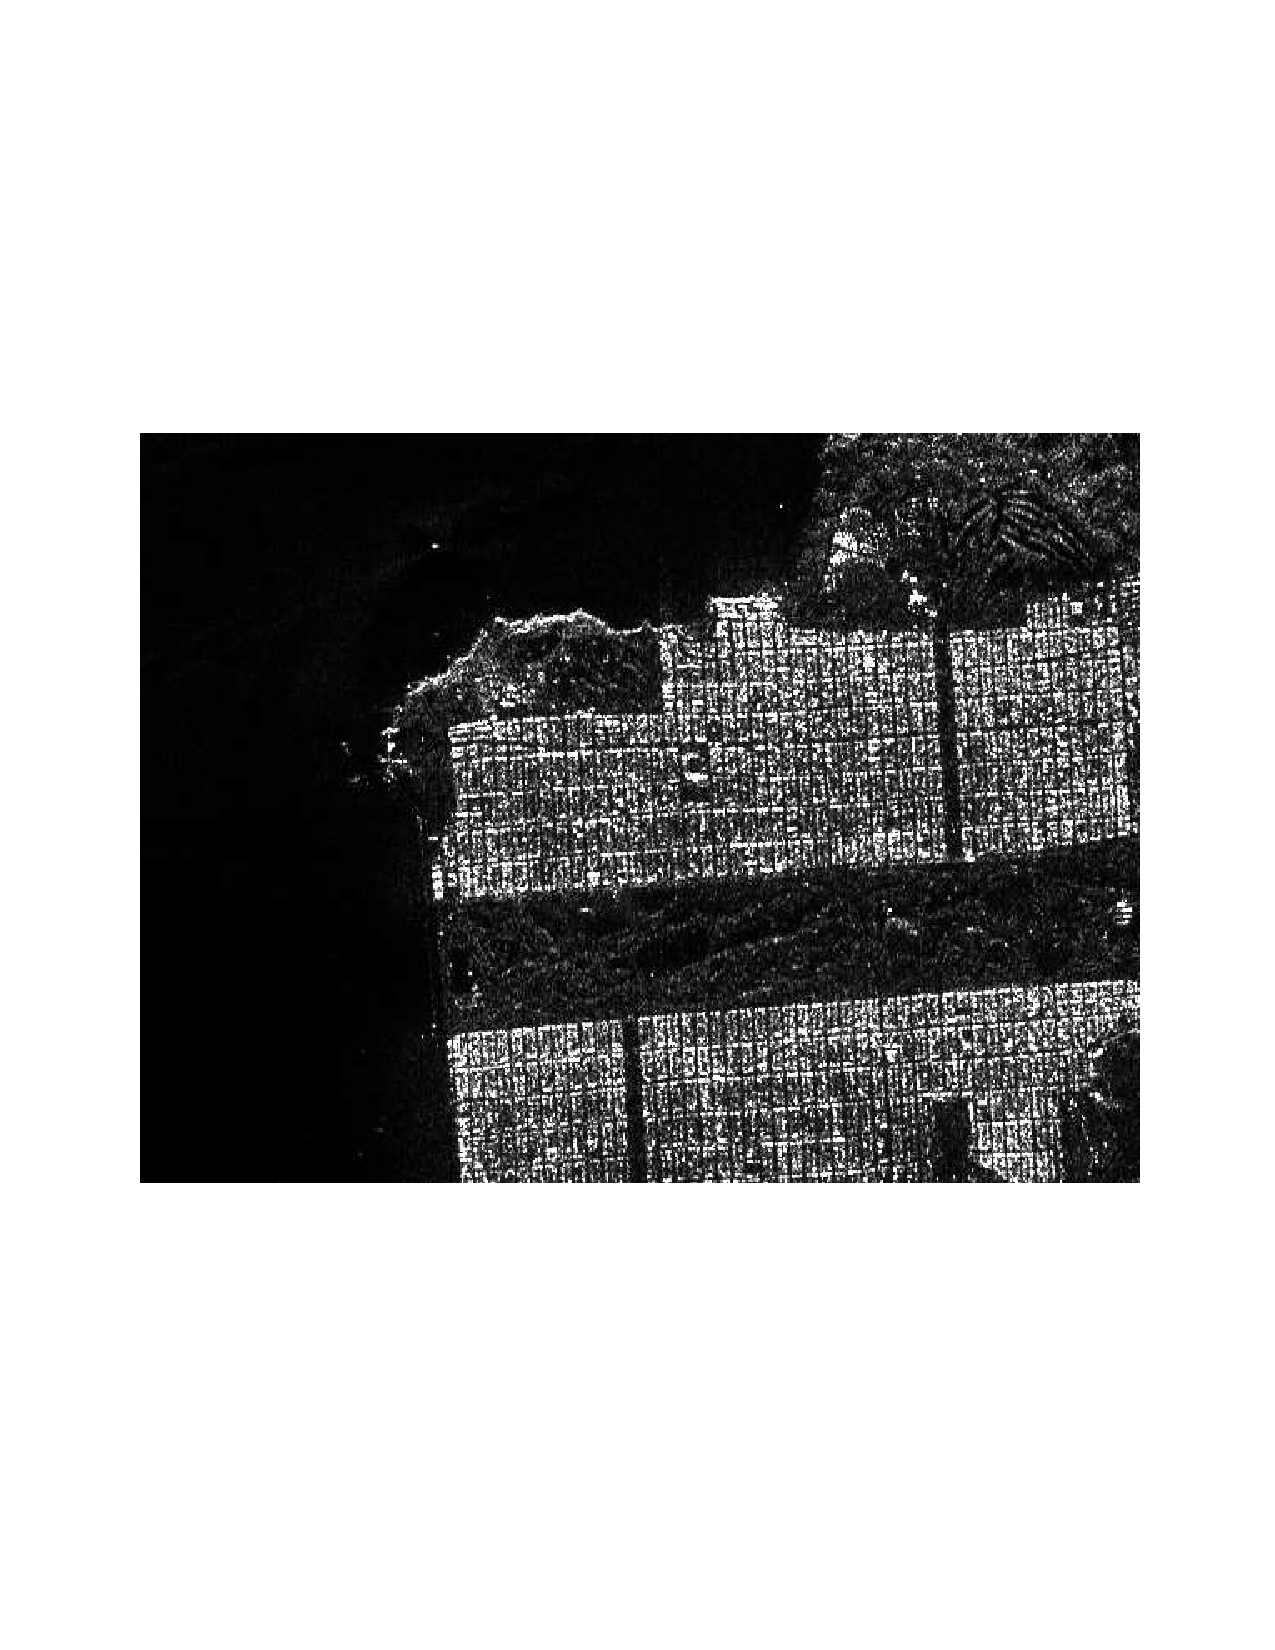
\includegraphics[width=\linewidth]{sf_hh.pdf}
\endminipage
\minipage{0.35\textwidth}
	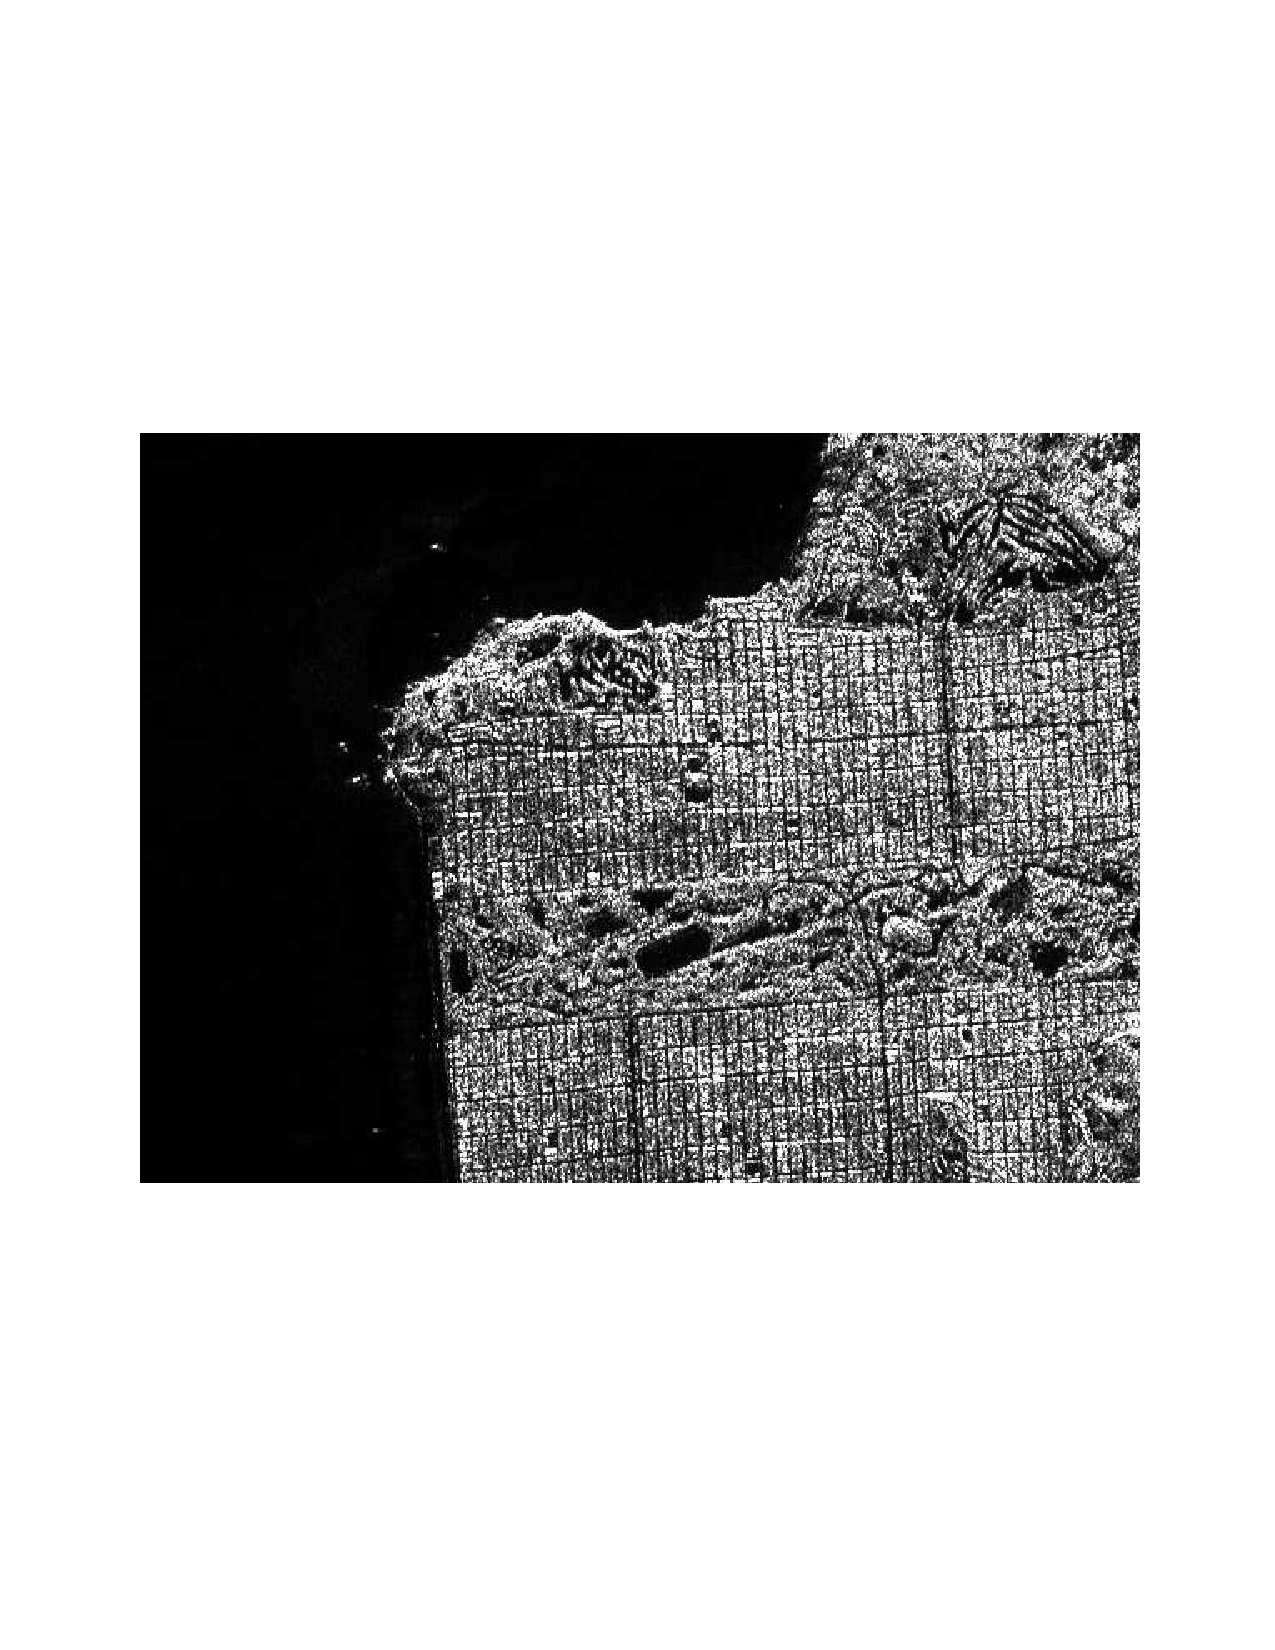
\includegraphics[width=\linewidth]{sf_vh.pdf}
\endminipage
%\centering
\minipage{0.35\textwidth}
	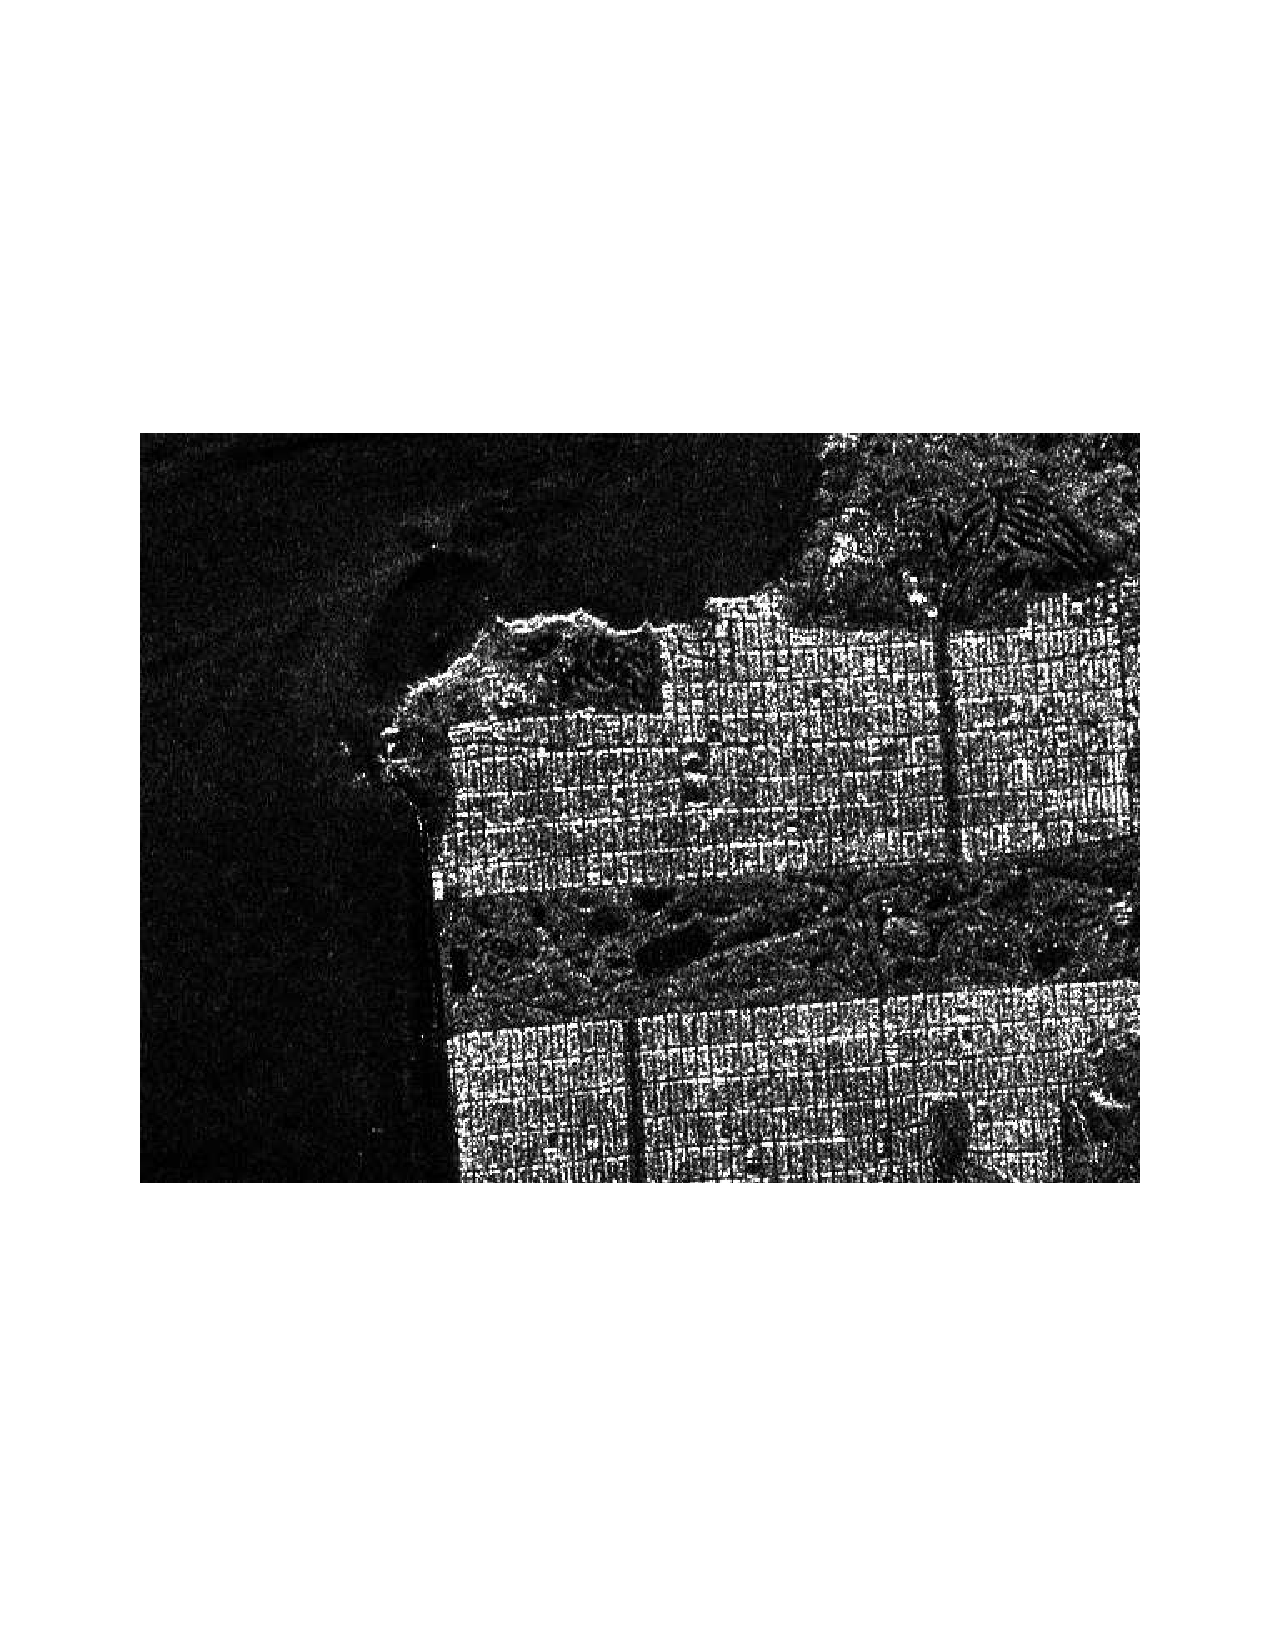
\includegraphics[width=\linewidth]{sf_vv.pdf}
\endminipage
  %      \vspace{-2.0cm}
	\caption{Imagem PolSAR com polarizações ($hh$, $hv$ e $vv$).}\label{cap_acf_sf_hh_hv_vv}
\end{figure}
\end{frame}

\begin{frame}{Imagem da baía de San Franscisco}
\begin{figure}[hbt]
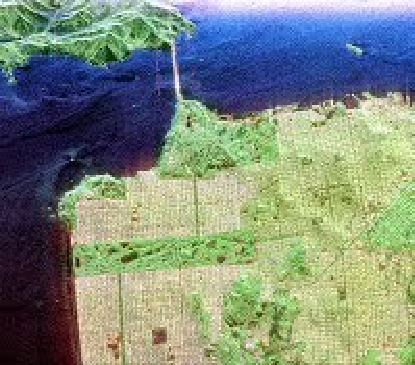
\includegraphics[scale=0.85]{polsar_teste.pdf}
\caption{Baía de São Francisco.}
\label{cap_acf_sf_pauli}
\end{figure}
\end{frame}

\section{Metodologia}
\begin{frame}{Modelagem estatística para dados PolSAR}
	
\begin{alertblock}{Equação de espalhamento.}
\begin{equation}\label{cap_acf_1}
 \left[
\begin{array}{c}
	E_{h}^{r}   \\
	E_{v}^{r}    \\
\end{array}
\right]
 = \frac{e^{\hat{\imath} kr}}{r}\left[
\begin{array}{cc}
	S_{hh}   & S_{hv}   \\
	S_{vh}   & S_{vv}   \\
\end{array}
\right]
 \left[
\begin{array}{c}
	E_{h}^{t}   \\
	E_{v}^{t}    \\
\end{array}
\right].
\end{equation}
\end{alertblock}
\end{frame}

\begin{frame}{Modelagem estatística para dados PolSAR}
	\begin{alertblock}{Matriz hermitiana.}
	\begin{itemize}
	\item Matriz de espalhamento.
	\begin{equation}\label{cap_acf_2}
\mathbf{S} = \left[
\begin{array}{cc}
	S_{hh}   & S_{hv}   \\
	S_{vh}   & S_{vv}   \\
\end{array}
\right],
\end{equation}
\item Teorema da reciprocidade
\begin{equation}\label{cap_acf_3}
\mathbf{s} = \left[
\begin{array}{c}
	S_{hh}      \\
    S_{vh}     \\
	S_{vv}      \\
\end{array}
\right].
\end{equation}
\end{itemize}
\end{alertblock}
\end{frame}

\begin{frame}[fragile]{Modelagem estatística para dados PolSAR}
      
  \alert{Probabilidade da distribuição Wishart.} 
%
\begin{equation}\label{cap_acf_4}
    f_{\mathbf{Z}}(\mathbf{Z};\Sigma,L)=\frac{L^{mL}|\mathbf{Z}|^{L-m}}{|\Sigma|^{L}\Gamma_m(L)} \exp(-L\traco{(\Sigma^{-1}\mathbf{Z})}), 
\end{equation}
    \alert{$\Gamma_m(L)$ - Função Gamma multivariada.}
\begin{equation}\label{cap_acf_5}
	\Gamma_m(L)=\pi^{\frac{1}{2}m(m-1)} \prod_{i=0}^{m-1}\Gamma(L-i),
\end{equation}
\alert{Matriz de covariância amostral estimada {\bf Z}.}
\begin{equation}\label{cap_acf_8}
\begin{array}{ccc}
    \mathbf{Z}&=&\frac{1}{L}\displaystyle{\sum_{i=1}^{L} {\mathbf{s}_i}{\mathbf{s}_i}^H}. \\
\end{array}
\end{equation}
\end{frame}

\begin{frame}{Detecão de bordas em imagens PolSAR}
  \begin{figure}[hbt]
\centering
	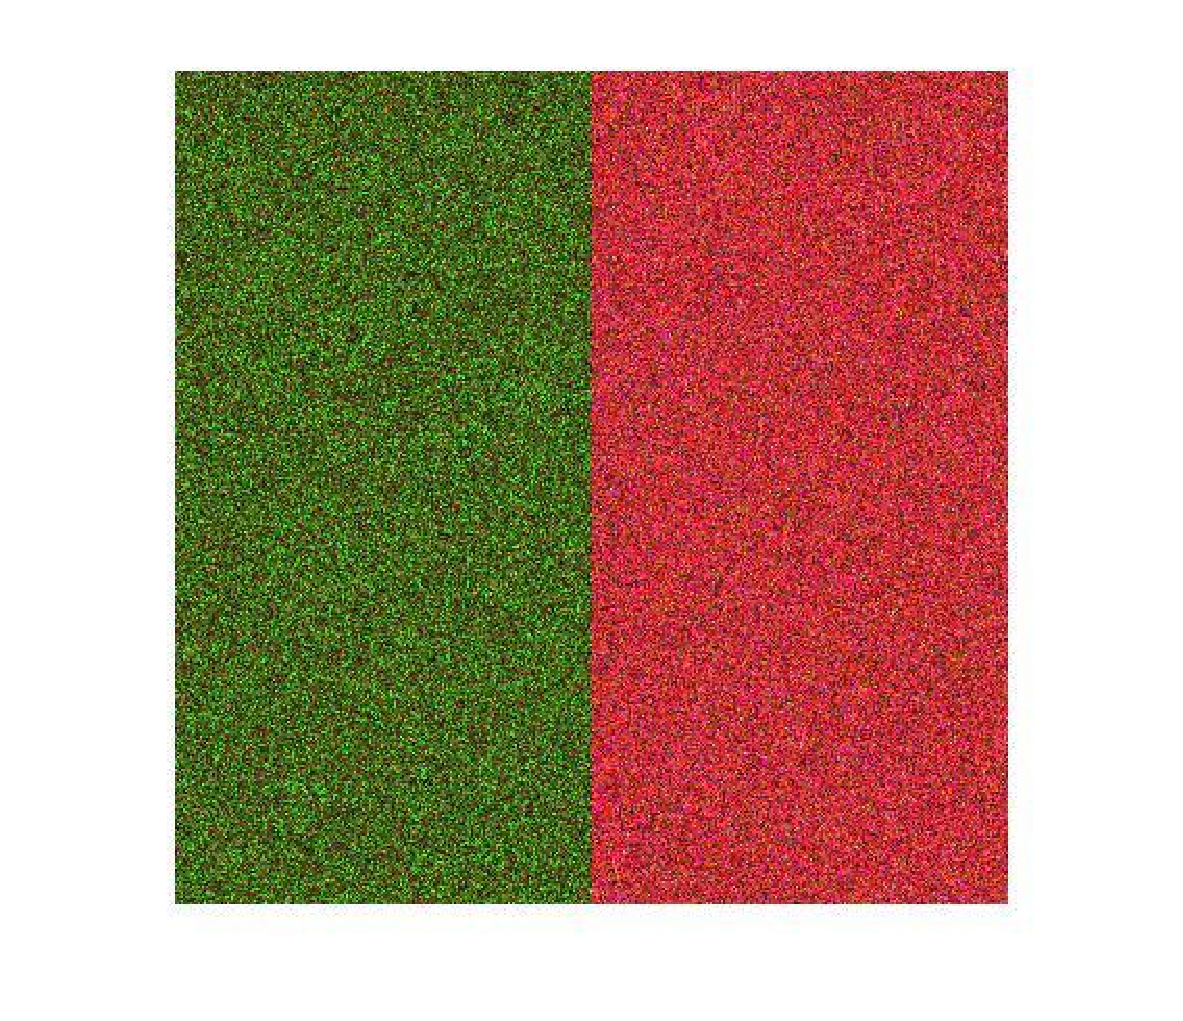
\includegraphics[scale=0.4]{phanton_nhfc_dec_pauli.pdf}
	\caption{Decomposição de Pauli para a phantom.}\label{cap_acf_fig01}
\end{figure}
\end{frame}

\begin{frame}{Detecão de bordas em imagens PolSAR}
\begin{figure}[hbt]
	\centering
	%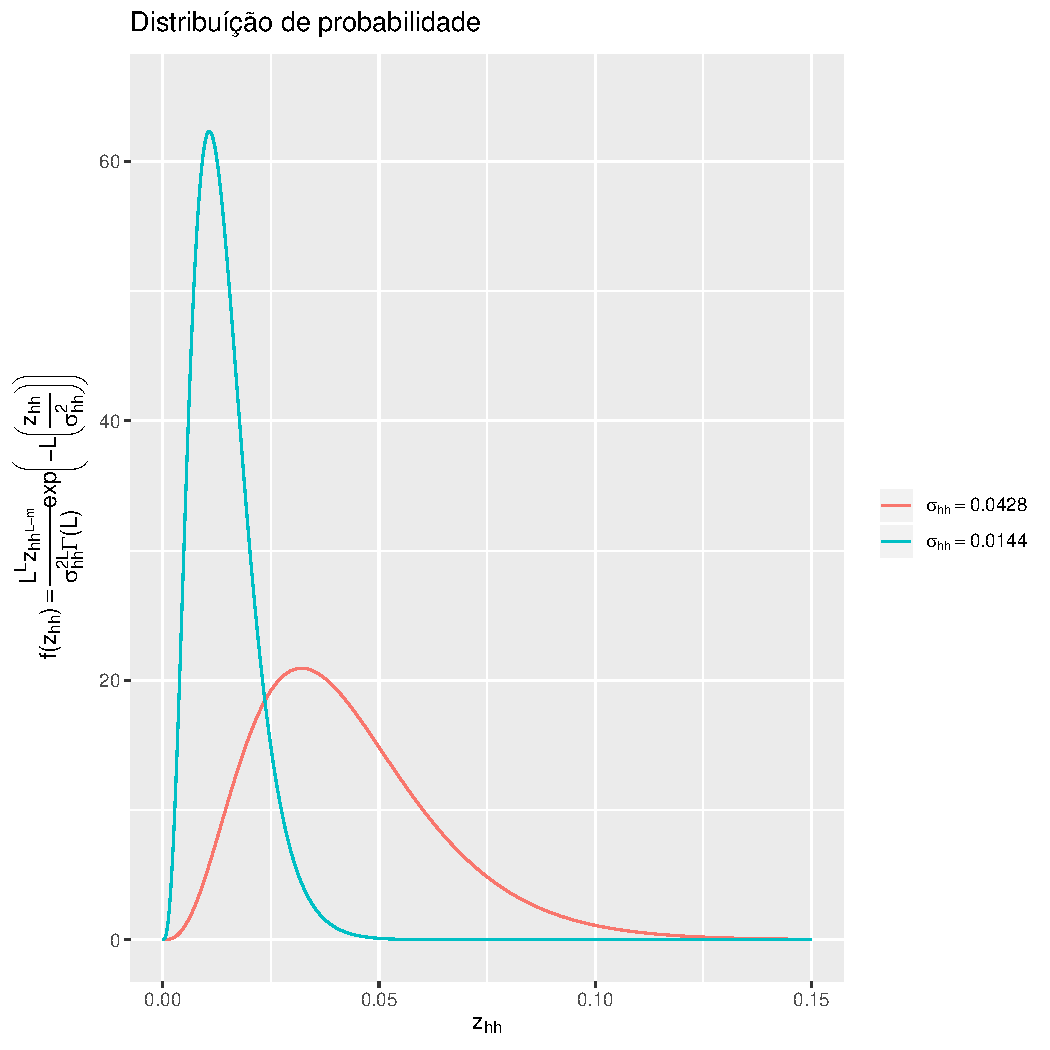
\includegraphics[scale = 1]{grafico_pdf_gamf_2017_sigma_hh.pdf}
  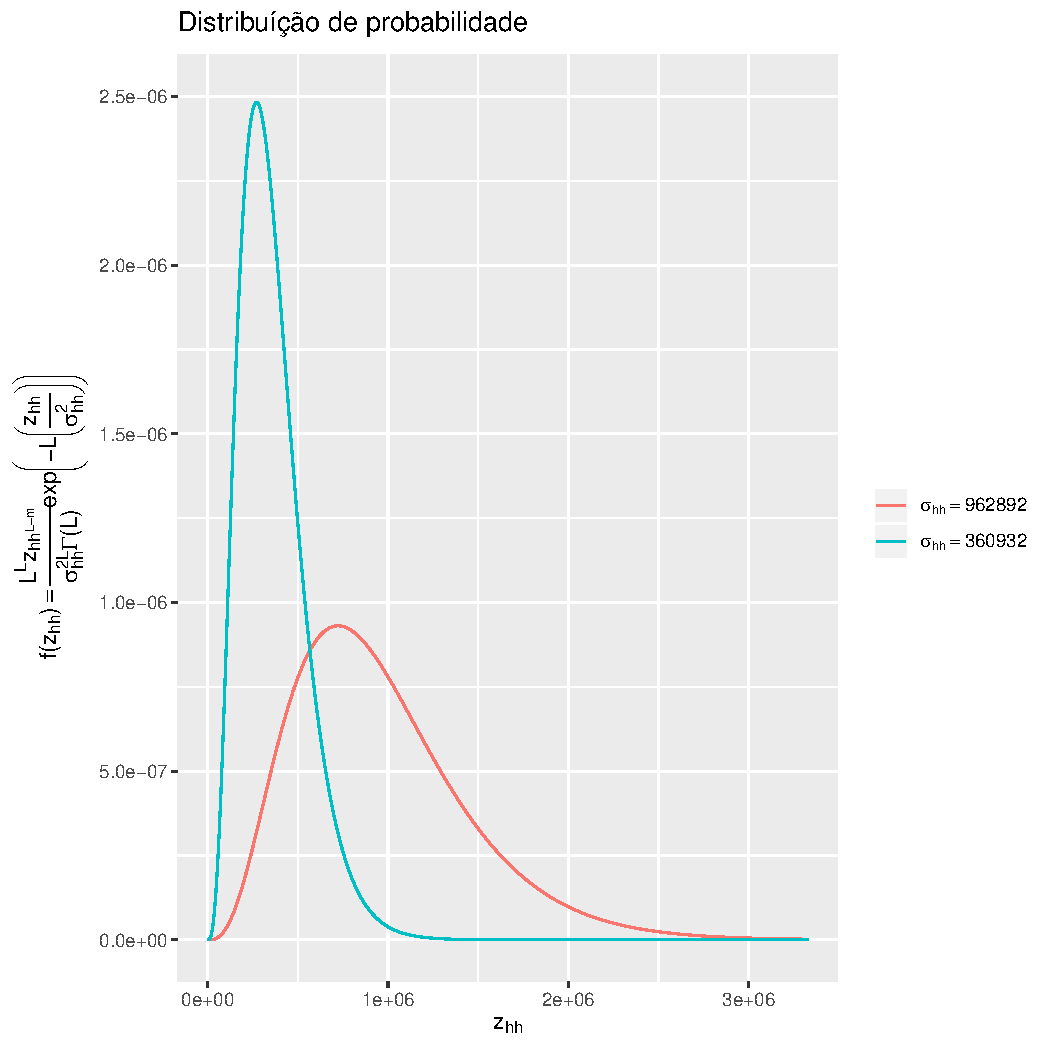
\includegraphics[scale = 0.4]{grafico_pdf_nhfc_2014_sigma_hh.pdf}
	\caption{Funções de densidade para dados simulados.}\label{cap_acf_fig02}
\end{figure}  
\end{frame}
\begin{frame}{Detecão de bordas em imagens PolSAR}
  \begin{alertblock}{Estimativa de máxima verossimilhança - \textbf{MLE}}
  \begin{itemize}
\item Função de verossimilhança
\begin{equation}\label{cap_acf_14}
    L(\theta;\mathbf{X}) = \prod_{i=1}^{n}f(x_i;\theta), 
\end{equation}
\item Função de log-verossimilhança
\begin{equation}\label{cap_acf_15}
	l(\theta;\mathbf{X})= \ln(L(\theta;\mathbf{X})) = \sum_{i=1}^{n}\ln(f(x_i;\theta)),
\end{equation}
\item 
\begin{equation}\label{cap_acf_16}
    \widehat{\theta}= \text{arg}\,\max\limits_{\theta\in\Theta}L(\theta;\mathbf{x}),
\end{equation}
\item
\begin{equation}\label{cap_acf_17}
    \widehat{\theta}= \text{arg}\,\max\limits_{\theta\in\Theta}l(\theta;\mathbf{x}).
\end{equation}
\end{itemize}
\end{alertblock}
\end{frame}

\begin{frame}{Detecão de bordas em imagens PolSAR}
\alert{Estimativa de máxima verossimilhança}
\begin{equation}\label{cap_acf_19}
	l(j)=\ln L(j)=\sum_{k=1}^{j}\ln f_{\mathbf{Z}}(\mathbf{Z}_{k}^{'};\Sigma_{A},L)+ \sum_{k=j+1}^{N}\ln f_{\mathbf{Z}}(\mathbf{Z}_{k}^{'};\Sigma_{B},L),
\end{equation}

\begin{equation}\label{cap_acf_20}
\widehat{\Sigma_{I}}(j) = \left\{
\begin{array}{lc}
	j^{-1}\sum_{k=1}^{j}\mathbf{Z}_{k}  & \mbox{se}\quad I=A,  \\
        (N-j)^{-1}\sum_{k=j+1}^{N}\mathbf{Z}_{k} & \mbox{se}\quad I=B, \\
\end{array}
\right.
\end{equation}
\begin{equation}\label{cap_acf_21}
\begin{array}{rcl}
	l(j)&=&N\left[-mL(1-\ln{\left(L\right)})-\ln{\left(\Gamma_m(L)\right)}\right]-L\left[j\ln{\left(|\widehat{\Sigma}_{A}(j)|\right)}\right. \\	
	&+&\left.(N-j)\ln{\left(|\widehat{\Sigma}_{B}(j)|\right)}\right], \\
	&+&(L-m)\sum_{k=1}^{N}\ln{\left(|\mathbf{Z}_{k}^{'}|\right)}, \\
\end{array}
\end{equation}

\begin{equation}\label{cap_acf_22}
	\widehat{\jmath}_{ML}=\text{arg}\max\limits_{j}l(j).  
\end{equation}
  
\end{frame}
\begin{frame}{Detecão de bordas em imagens PolSAR}
  \begin{figure}[hbt]
\minipage{0.30\textwidth}
  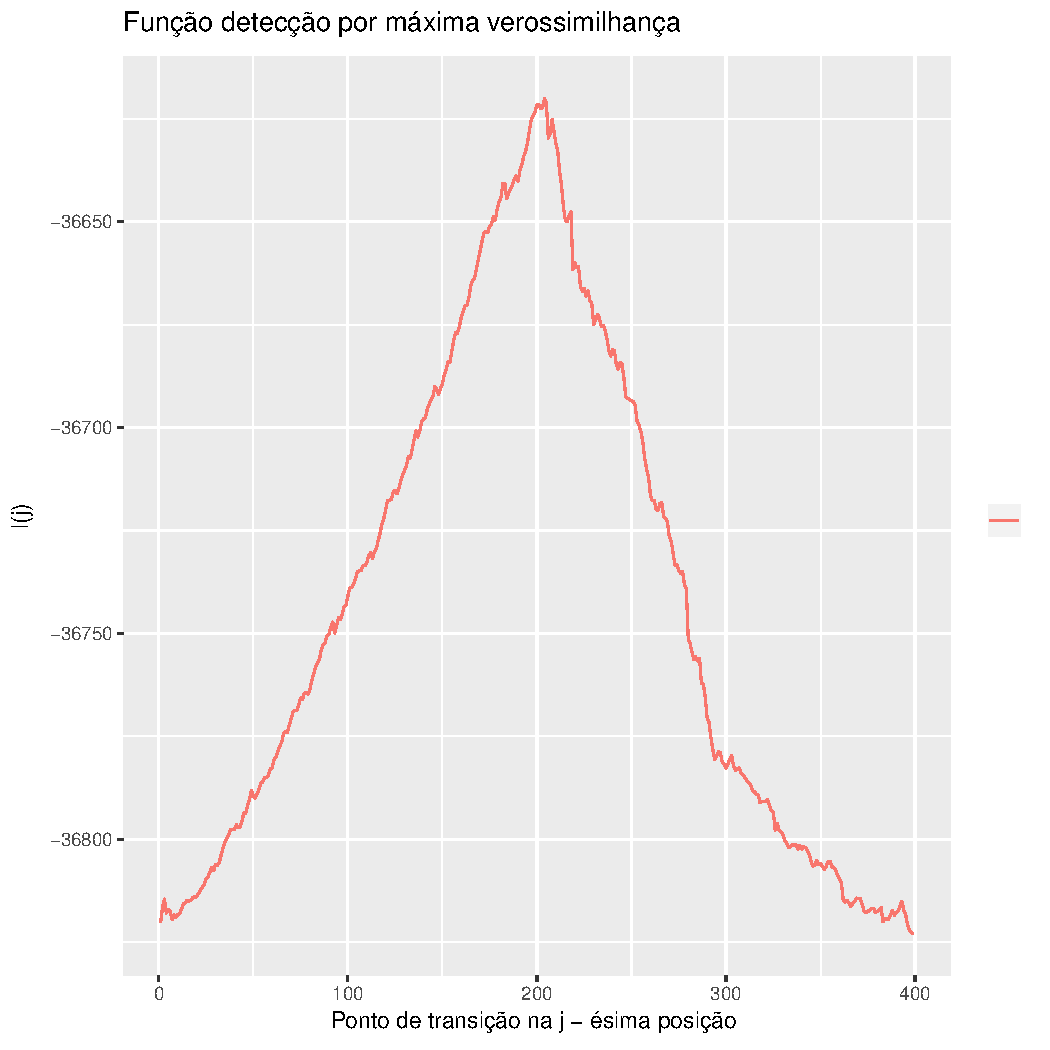
\includegraphics[width=\linewidth]{grafico_l_nhfc_2014_sigmahh.pdf}
	\caption{Função $l(j)$ para o canal $I_{HH}$.}\label{cap_acf_fig04}
\endminipage\hfill
\minipage{0.30\textwidth}
  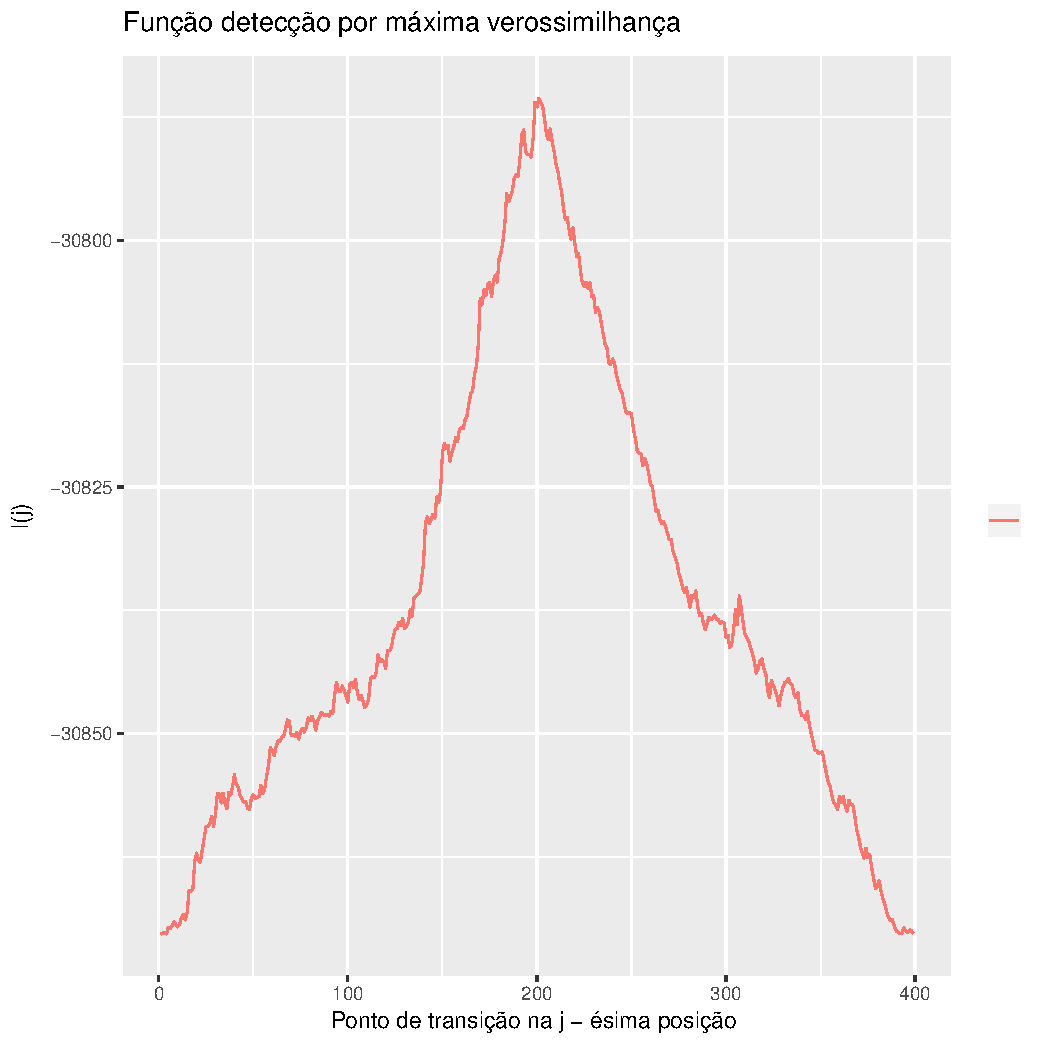
\includegraphics[width=\linewidth]{grafico_l_nhfc_2014_sigmahv.pdf}
	\caption{Função $l(j)$ para o canal $I_{HV}$.}\label{cap_acf_fig05}
\endminipage\hfill
\minipage{0.30\textwidth}
  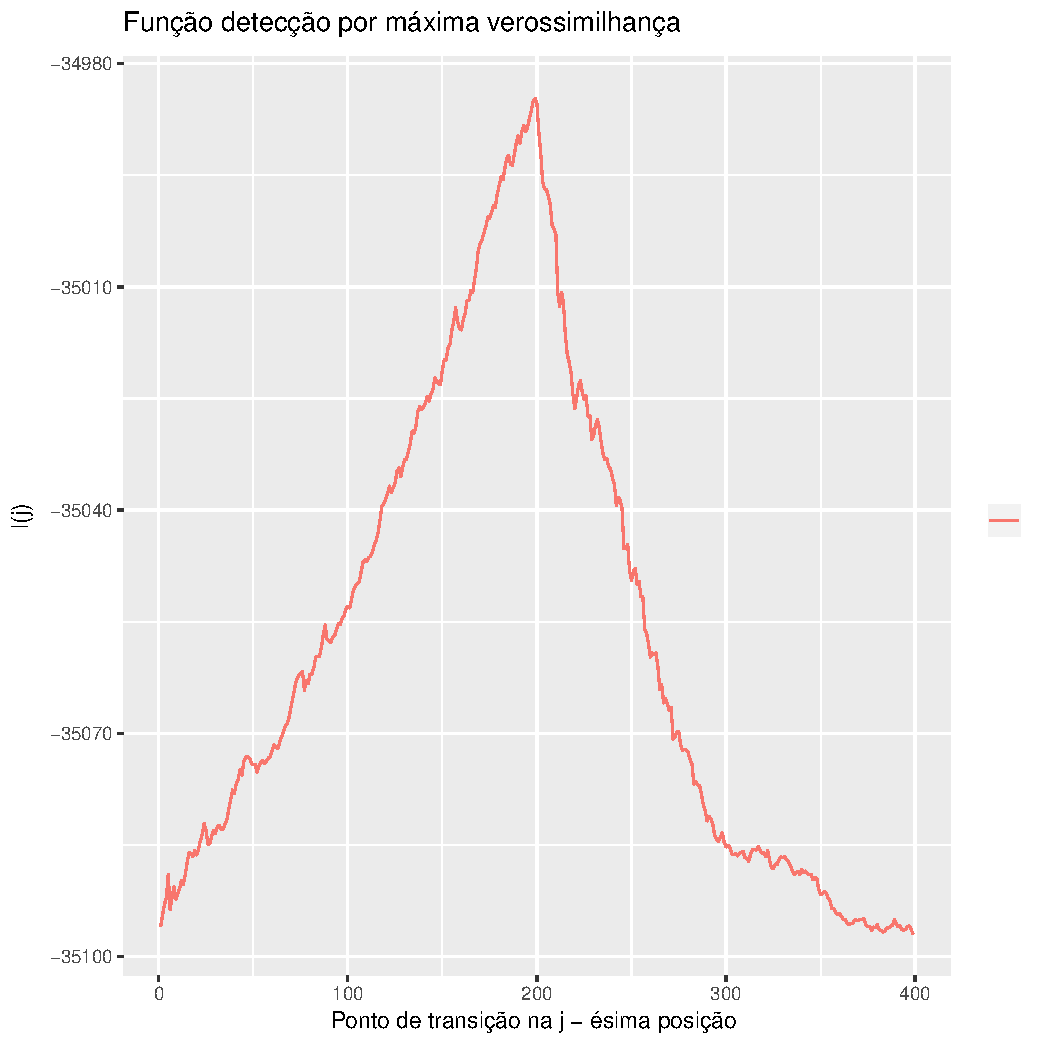
\includegraphics[width=\linewidth]{grafico_l_nhfc_2014_sigmavv.pdf}
	\caption{Função $l(j)$ para o canal $I_{VV}$.}\label{cap_acf_fig06}
\endminipage\hfill
\end{figure}
\end{frame}
\section{Resultados numéricos}
\begin{frame}{Detecão de bordas em imagens PolSAR}
\begin{alertblock}{Otimização}
  \begin{itemize}
\item GenSA;
\item Generalized Simulated Annealing.
\end{itemize}
\end{alertblock}
\end{frame}

\begin{frame}{Resultados numéricos}
\alert{GenSA aplicado em $l(j)$ nos respectivos canais.}
\begin{figure}[hbt]
\minipage{0.3\textwidth}
  \fbox{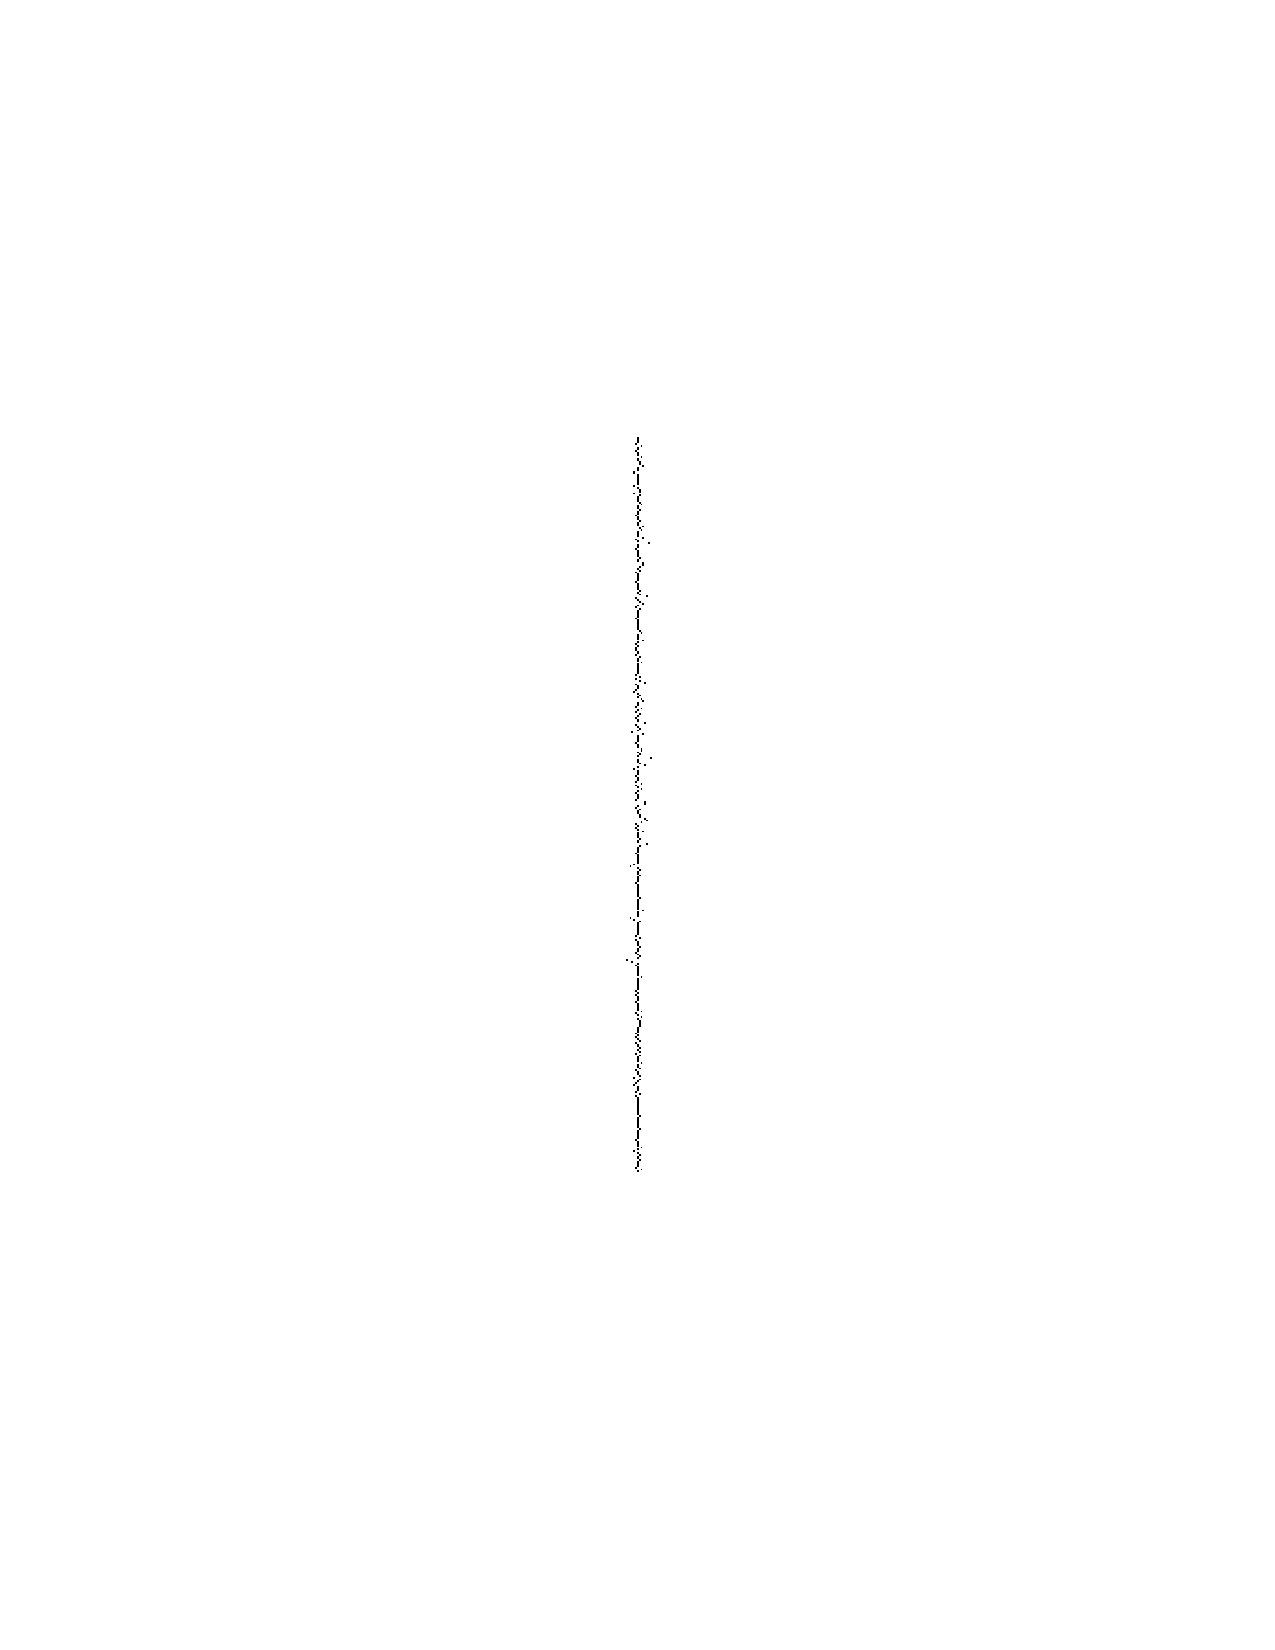
\includegraphics[width=\linewidth]{ev_hh_nhfc_2014.pdf}}
\caption{Evidências de bordas no canal $I_{HH}$.}\label{cap_acf_fig07}
\endminipage\hfill
\minipage{0.3\textwidth}
\fbox{ 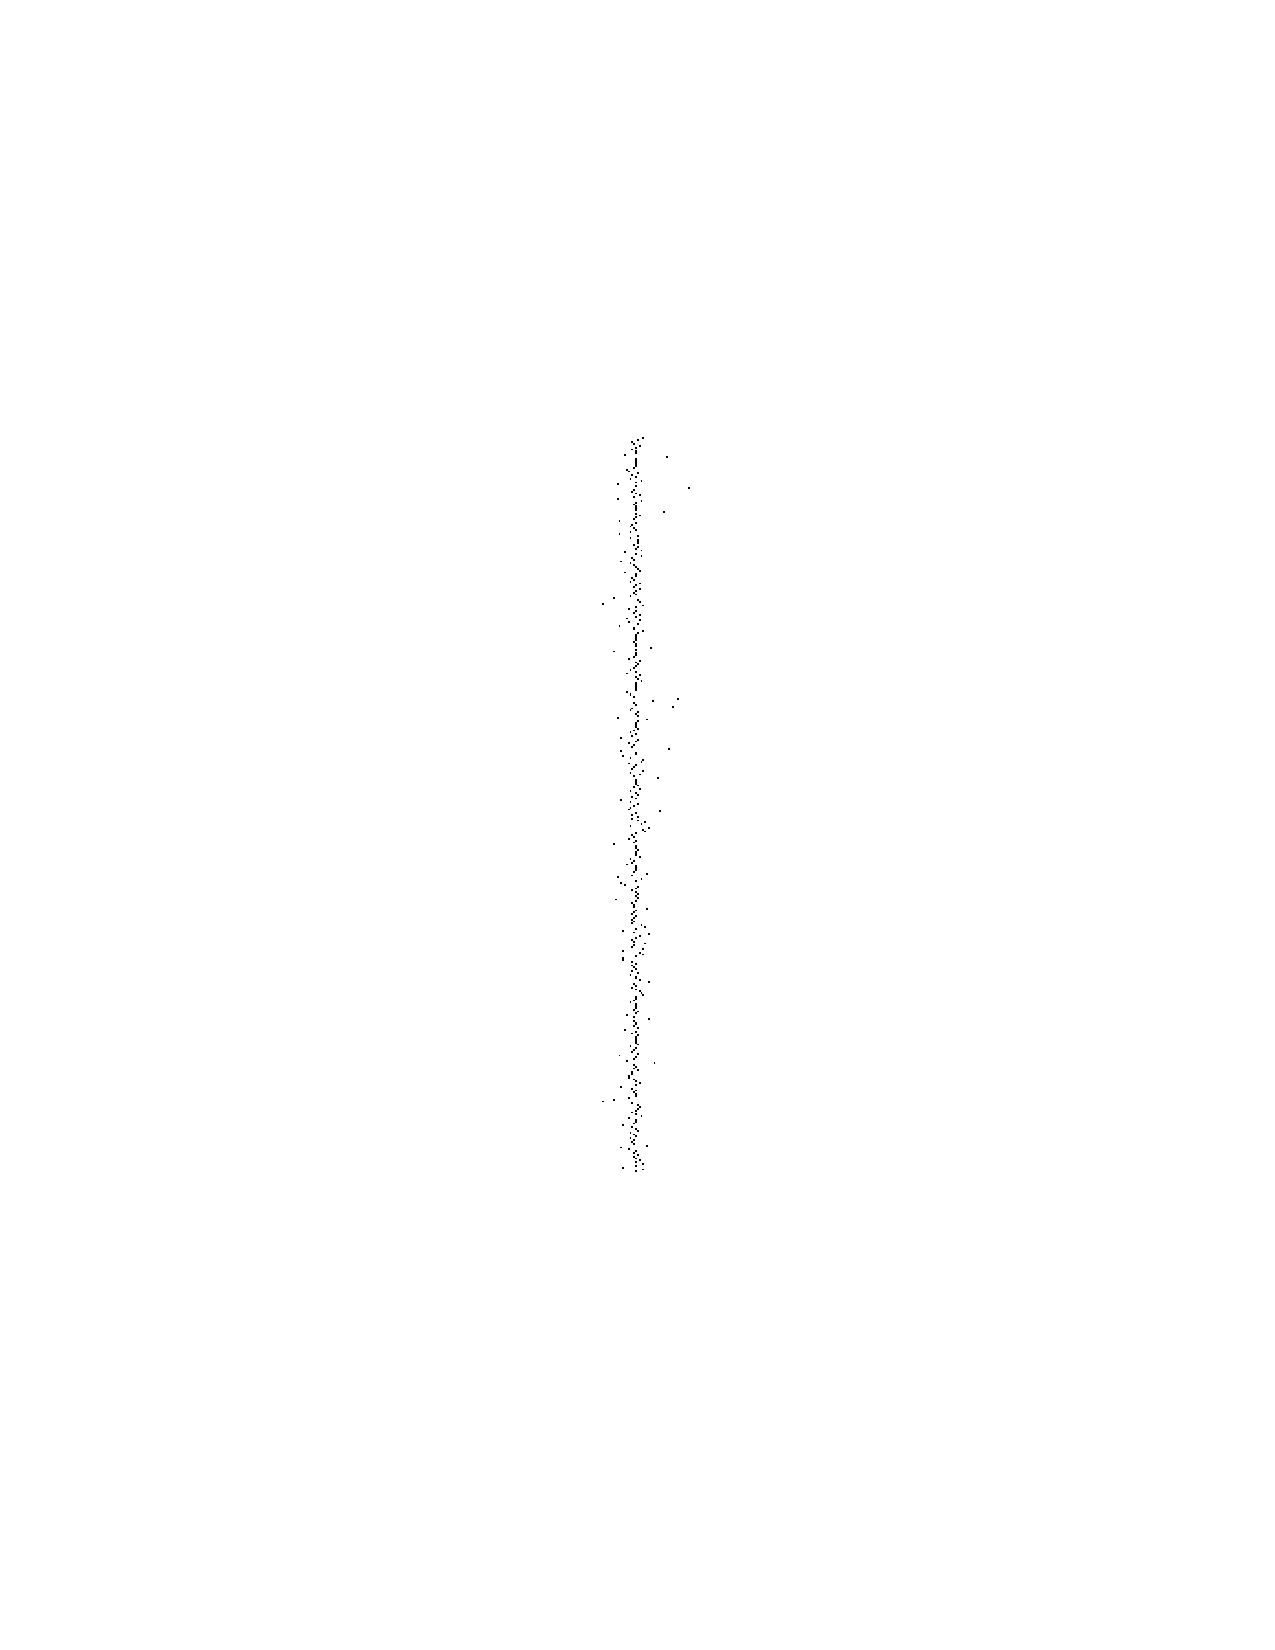
\includegraphics[width=\linewidth]{ev_hv_nhfc_2014.pdf}}
\caption{Evidências de bordas no canal $I_{HV}$.}\label{cap_acf_fig08}
\endminipage\hfill
\minipage{0.3\textwidth}
\fbox{ 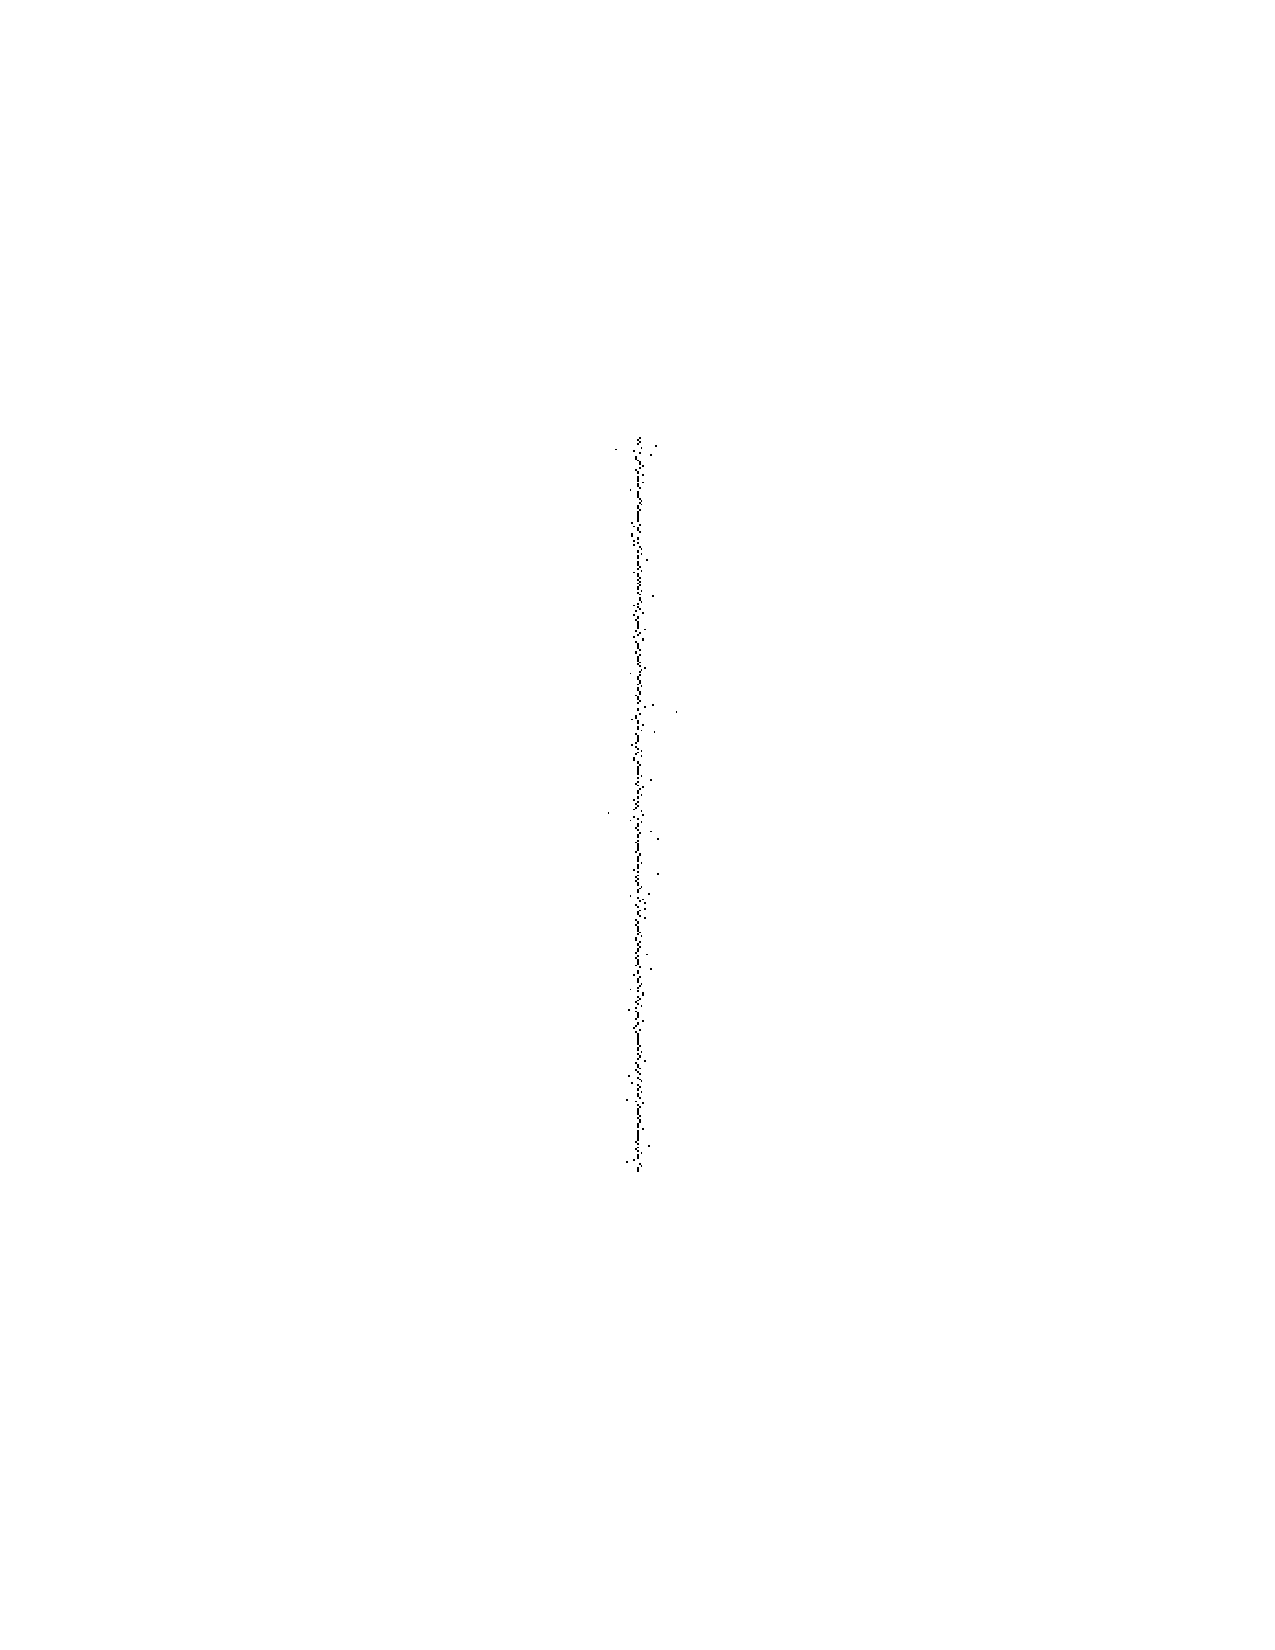
\includegraphics[width=\linewidth]{ev_vv_nhfc_2014.pdf}}
\caption{Evidências de bordas no canal $I_{VV}$.}\label{cap_acf_fig09}
\endminipage\hfill
\end{figure}
\end{frame}
\begin{frame}{Resultado numéricos}
\alert{Fusão de evidências de bordas}
  \begin{equation}\label{cap_acf_27}
\begin{array}{lll}
	F_{m}^{ev} &=&\frac{1}{K}\displaystyle{\sum_{k=1}^{K}ev_k}. 
\end{array}
\end{equation}
\end{frame}

\begin{frame}{Resultados numéricos}
\alert{Fusão de evidências e Quadrados mínimos}
\begin{figure}[hbt]
\minipage{0.40\textwidth}
	\fbox{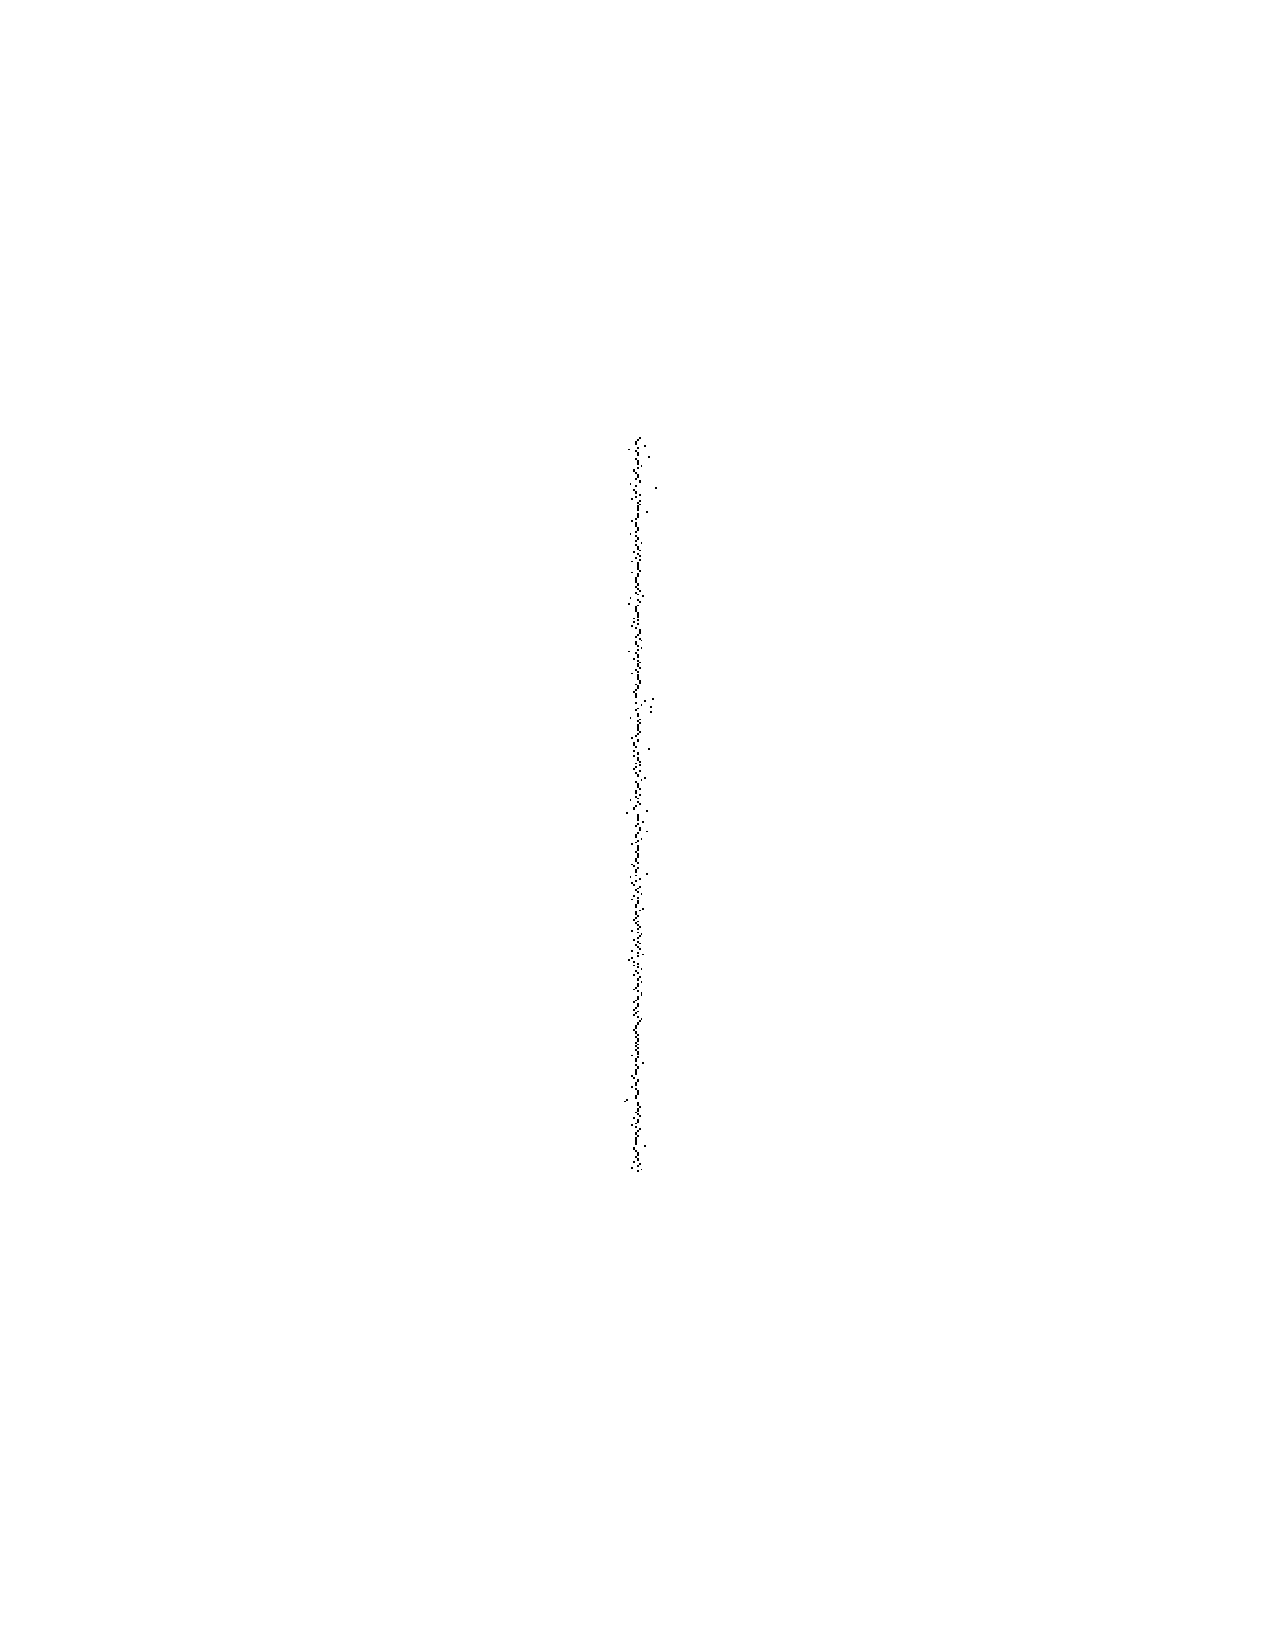
\includegraphics[width=\linewidth]{fusao_soma_ev_hh_hv_vv_nhfc.pdf}}
	\caption{Fusão de evidências para os canais $\left(I_{hh}, I_{hv}, I_{vv}\right)$.}
\label{cap_acf_fig11}
\endminipage\hfill
\minipage{0.40\textwidth}
\fbox{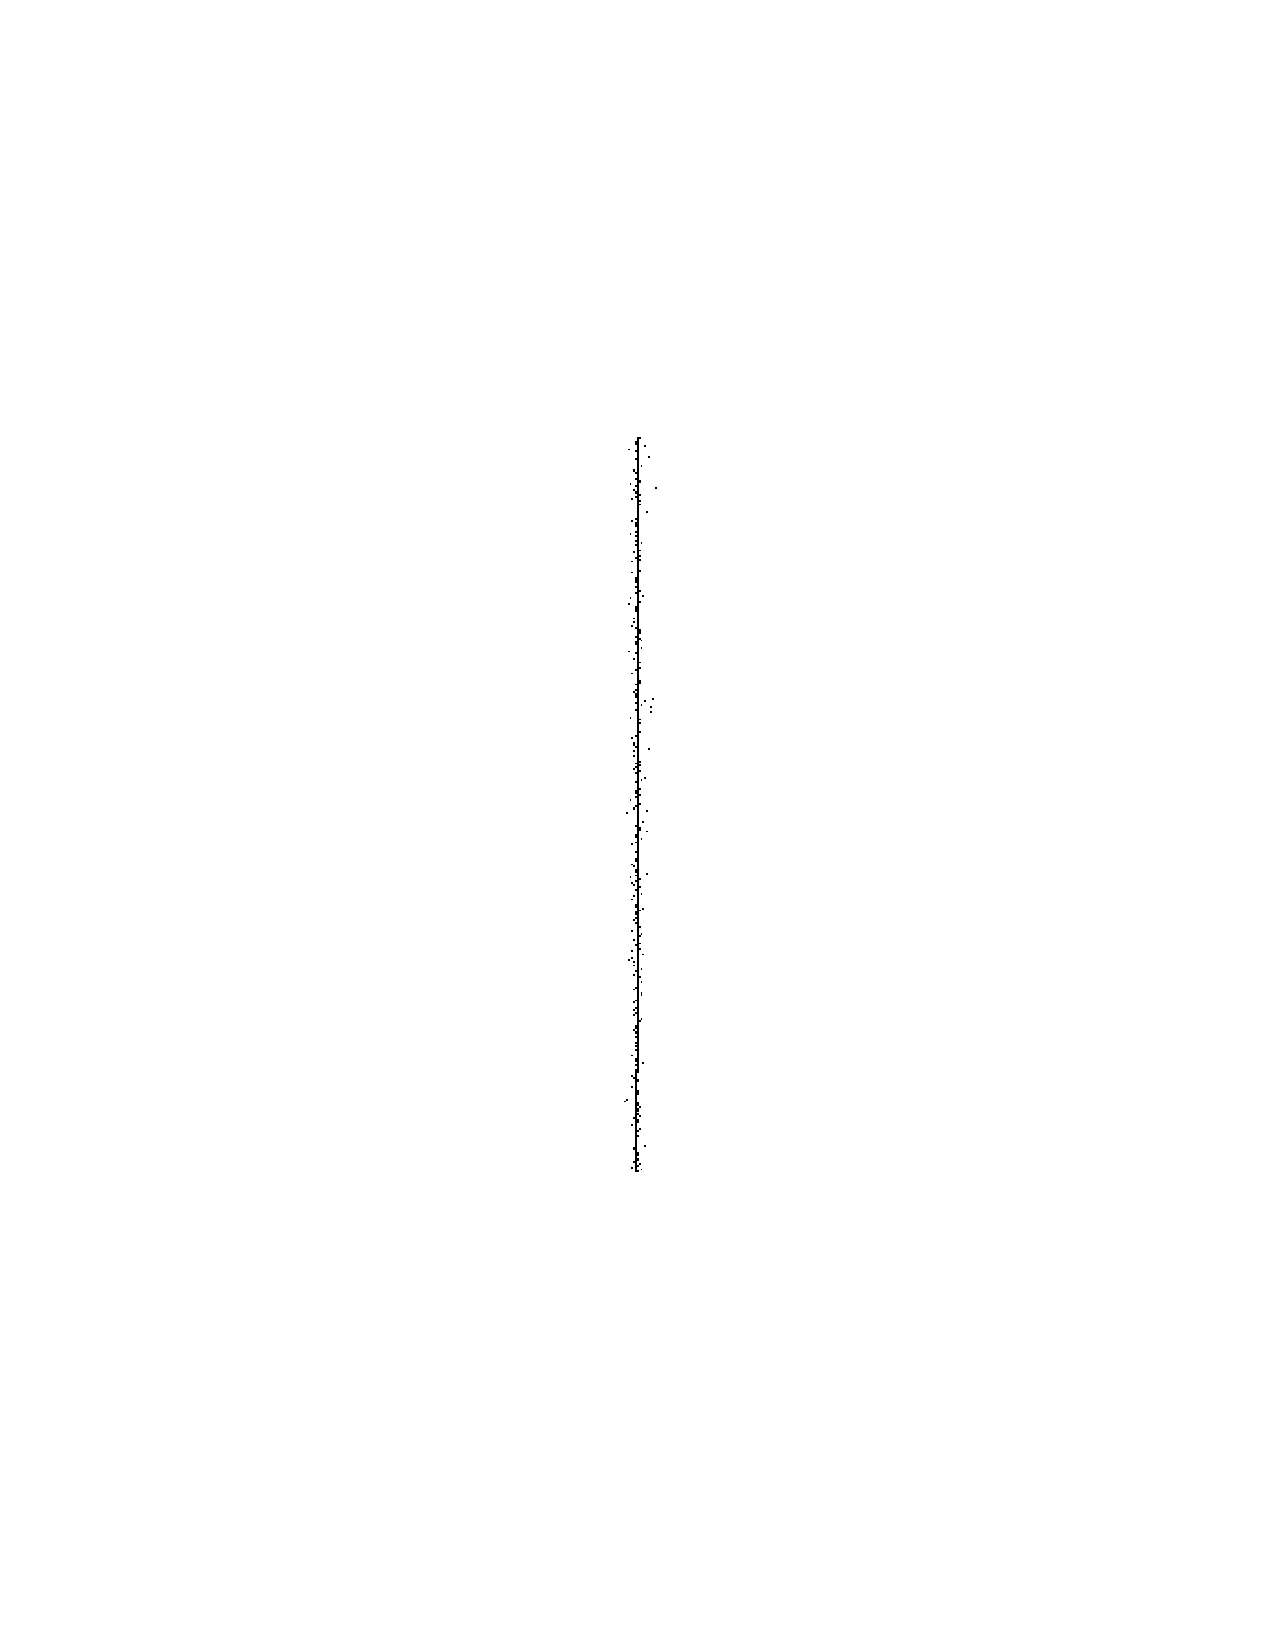
\includegraphics[width=\linewidth]{fusao_ls_nhfc.pdf}}	
\caption{Método dos quadrados mínimos.}
\label{cap_acf_fig12}
\endminipage\hfill
\end{figure}
\end{frame}
\begin{frame}{Resultados numéricos}
\begin{figure}[hbt]
\minipage{0.475\textwidth}
	\fbox{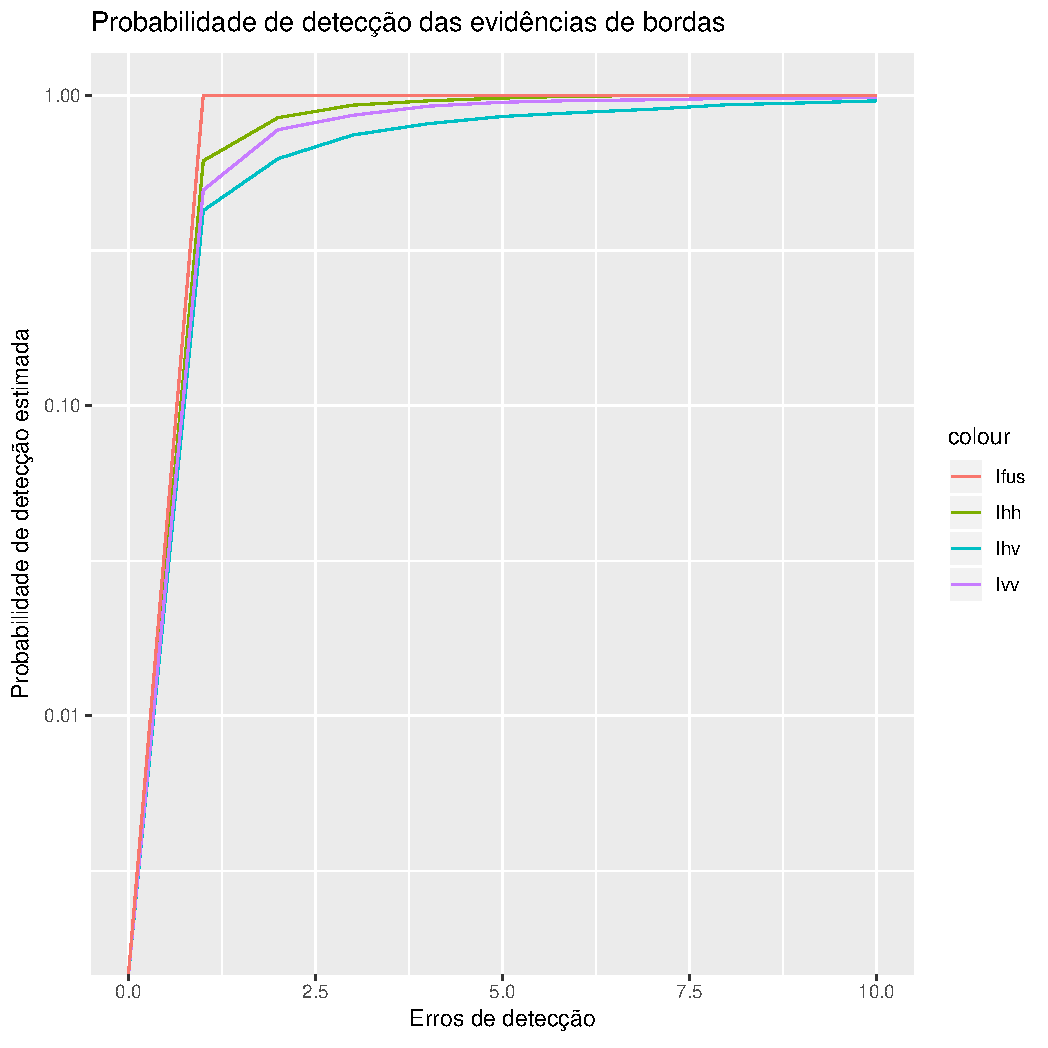
\includegraphics[width=\linewidth]{metricas_ihh_ivh_ivv_ils_nhfc.pdf}}
	\caption{Probabilidade de detecção de borda com fusão de evidências nos respectivos canais.}
\label{cap_acf_fig13}
\endminipage\hfill
\minipage{0.475\textwidth}
\fbox{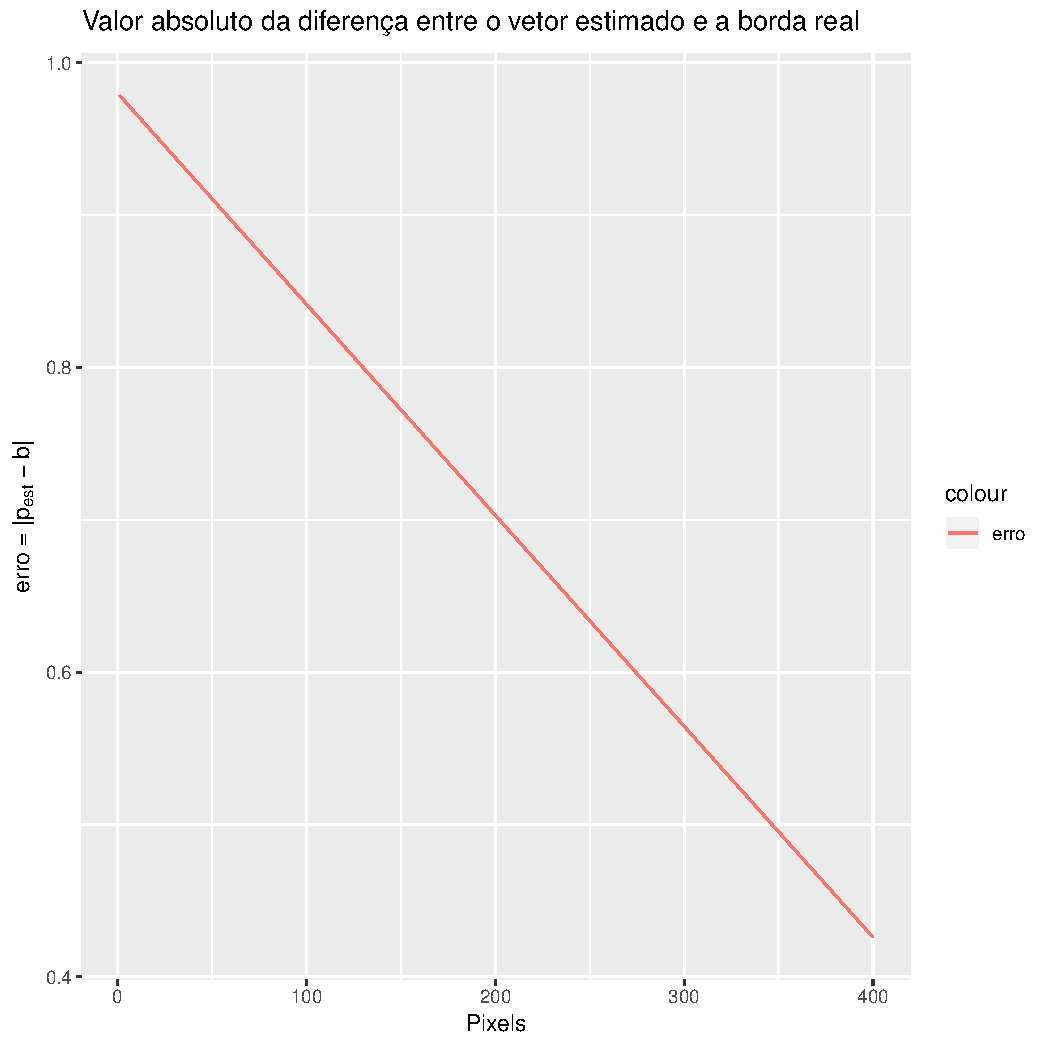
\includegraphics[width=\linewidth]{fusao_ls_erro_nhfc.pdf}}	
	\caption{Valor absoluto da diferença entre o vetor estimado da fusão de evidências e a borda real.}
\label{cap_acf_fig14}
\endminipage\hfill
\end{figure}
\end{frame}

\begin{frame}{Resultados numéricos}
\begin{figure}[hbt]
\minipage{0.45\textwidth}
	\fbox{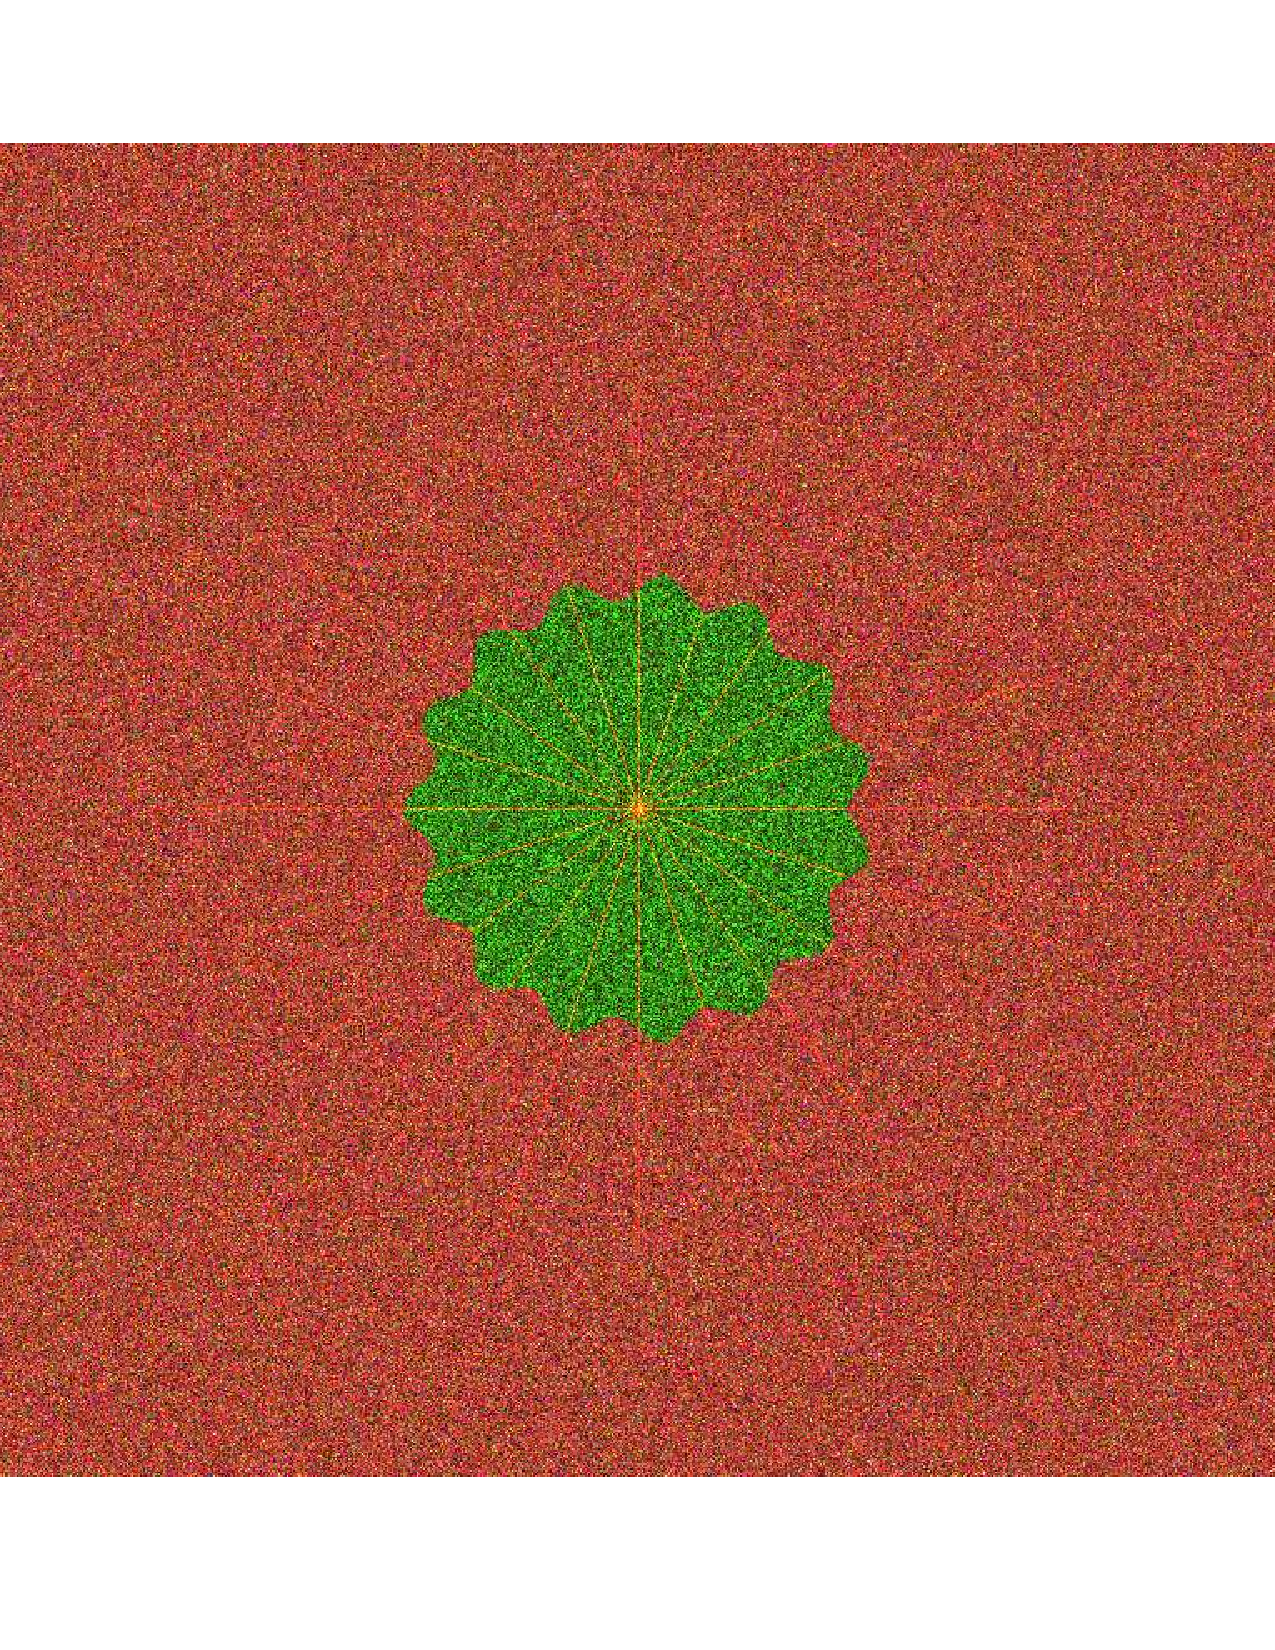
\includegraphics[width=\linewidth]{flor_15_133_8_pauli.pdf}}
	\caption{Imagem flor simulada com parâmetros $\beta = 15$, $\delta = 133$ e $\nu = 8$ .}
\label{cap_acf_fig15}
\endminipage\hfill
\minipage{0.45\textwidth}
\fbox{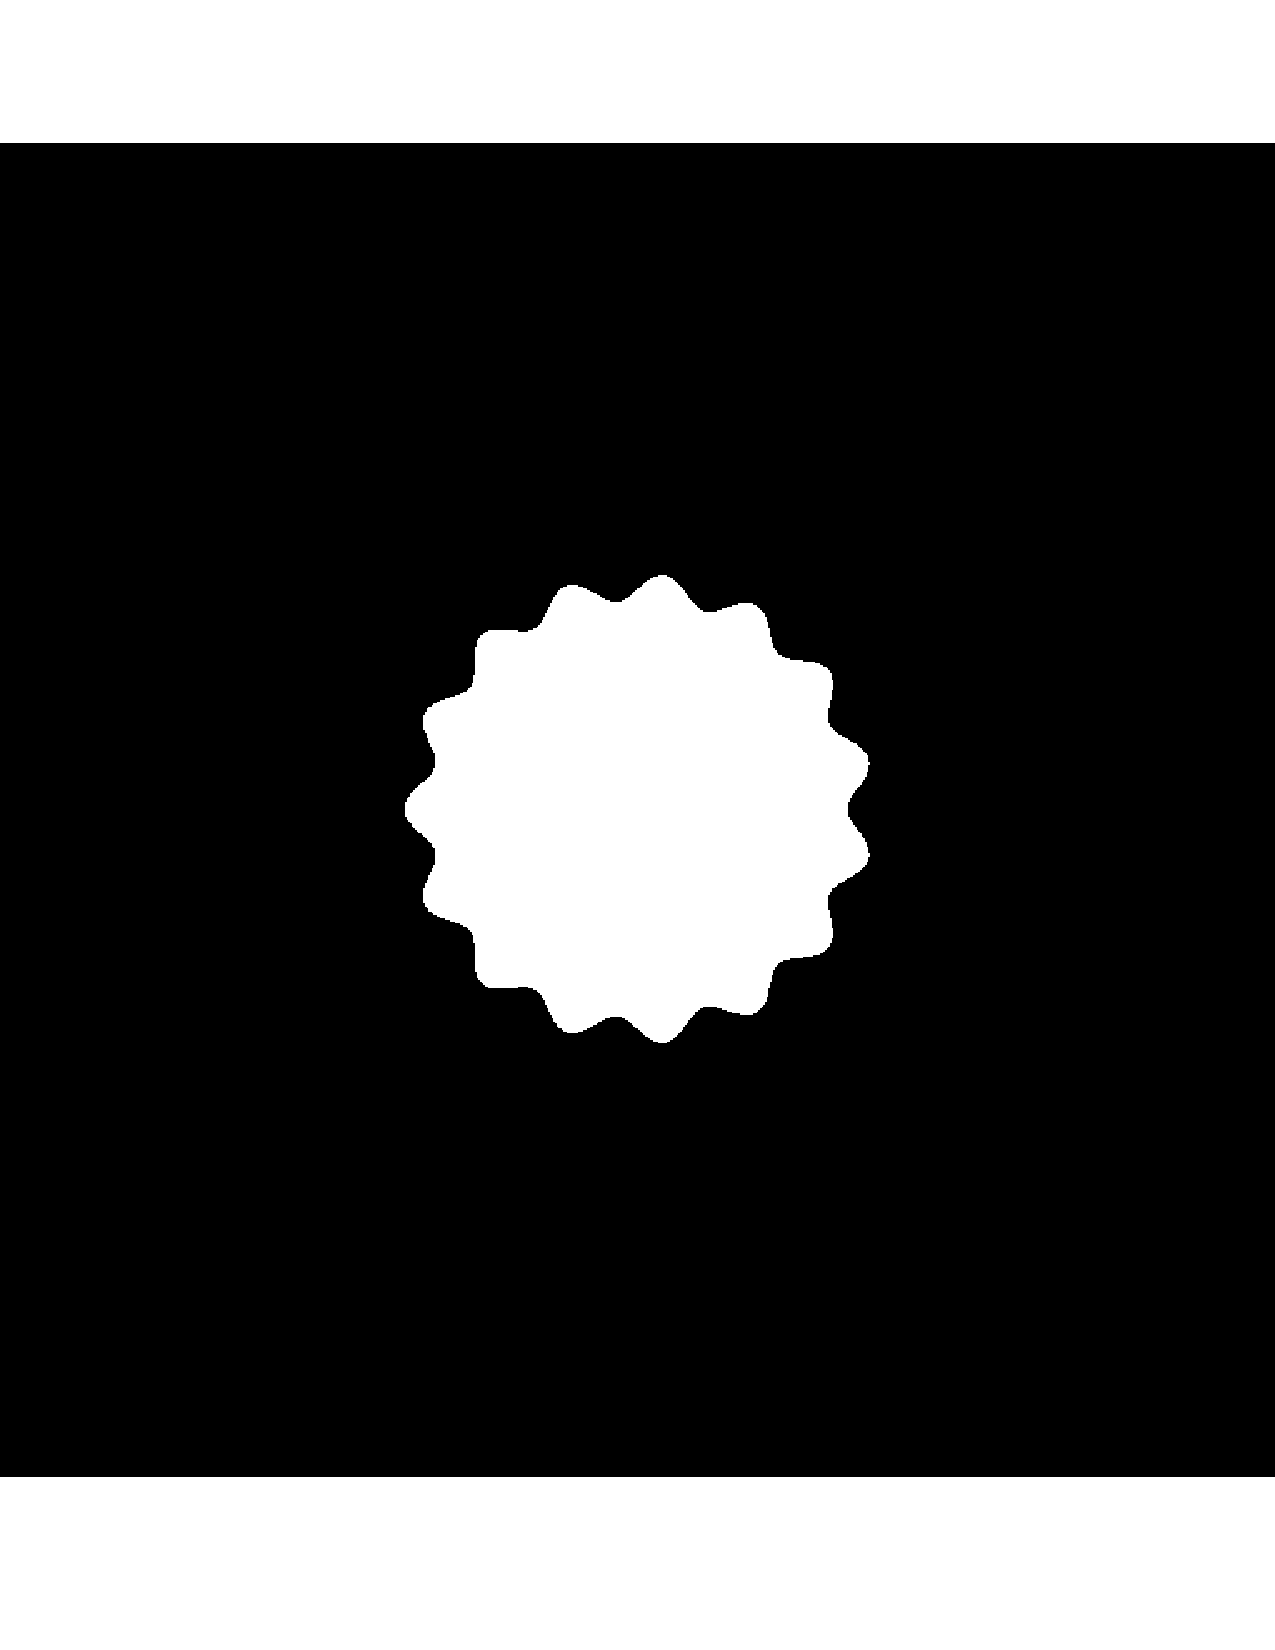
\includegraphics[width=\linewidth]{flor_15_133_8_bin.pdf}}	
	\caption{Imagem flor simulada binária com $\beta = 15$, $\delta = 133$ e $\nu = 8$ .}
\label{cap_acf_fig16}
\endminipage
\end{figure}
\end{frame}

\begin{frame}{Resultados numéricos}
\begin{figure}[hbt]
\minipage{0.3\textwidth}
\fbox{  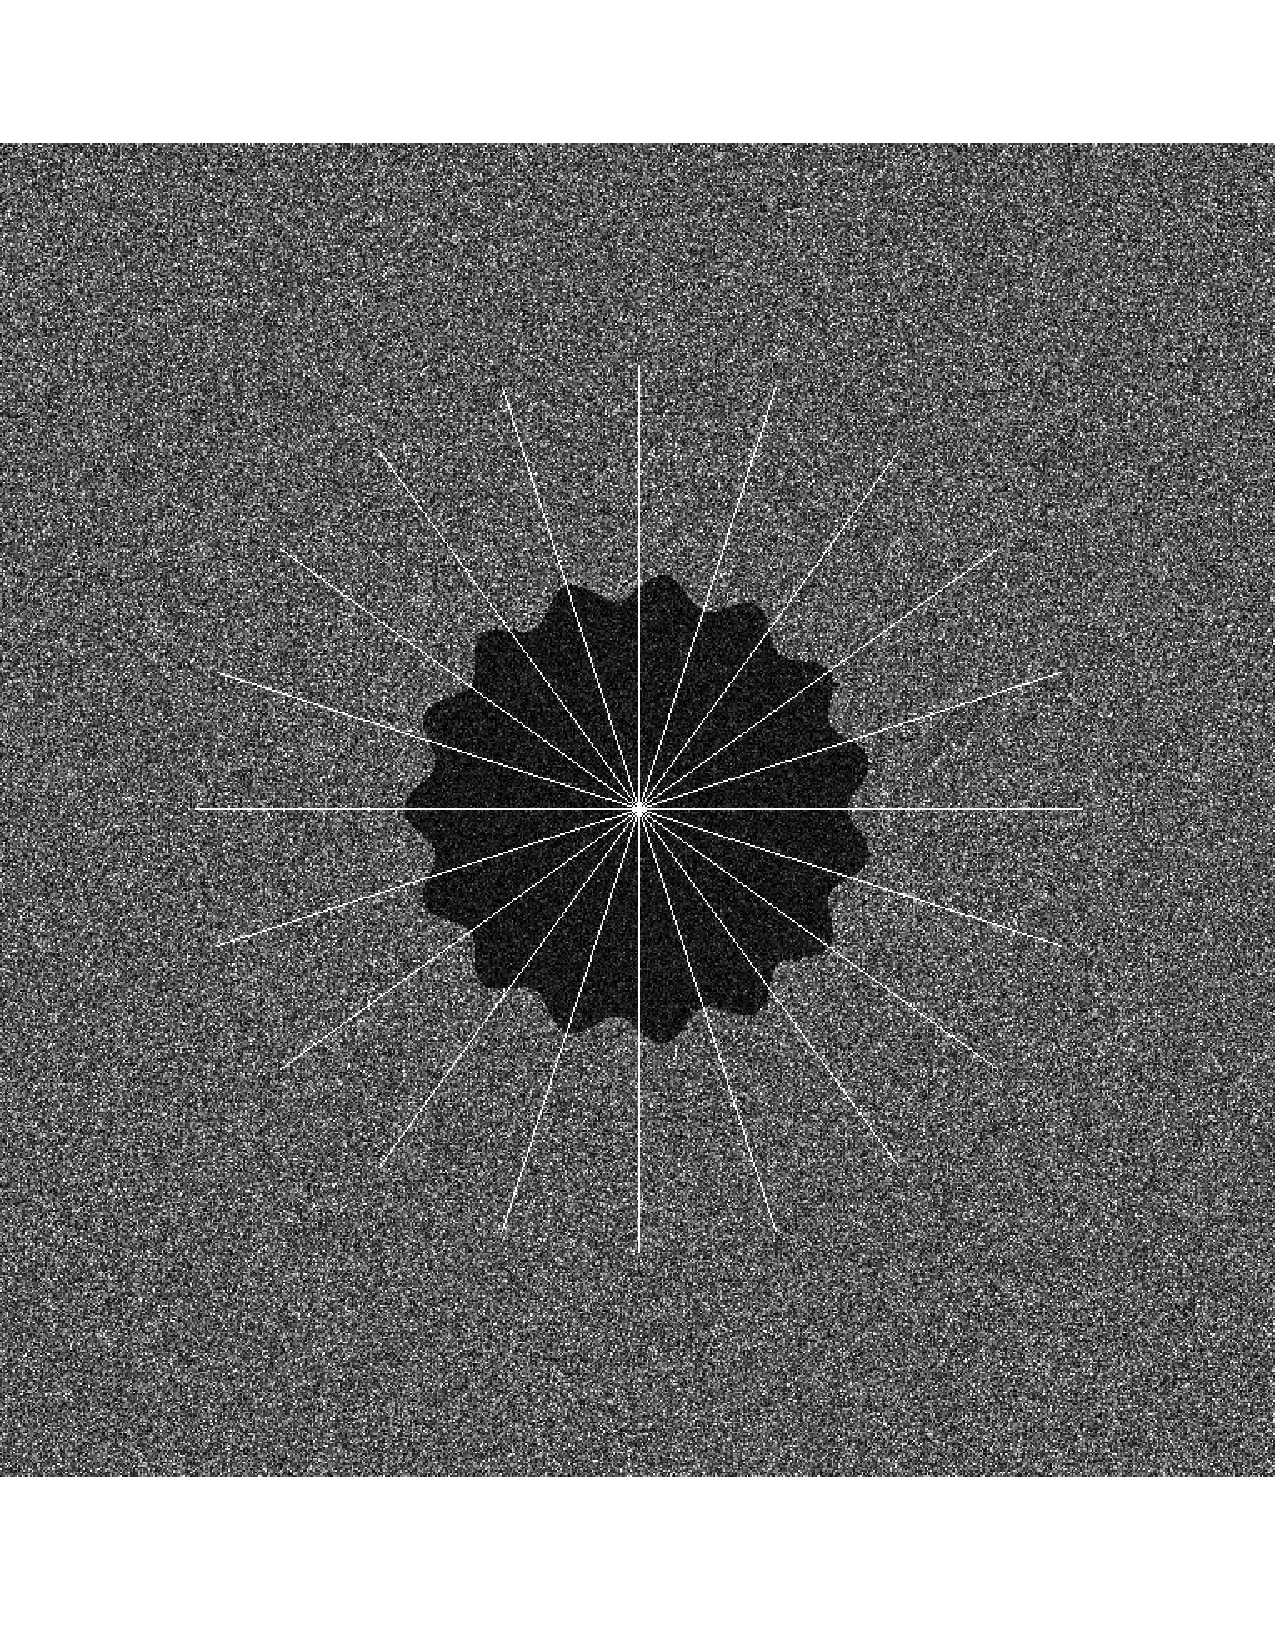
\includegraphics[width=\linewidth]{flor_15_133_8_hh.pdf}}
	\caption{Imagem flor simulada canal $I_{hh}$ com $\beta = 15$, $\delta = 133$ e $\nu = 8$ .}
\endminipage\hfill
\minipage{0.3\textwidth}
\fbox{ 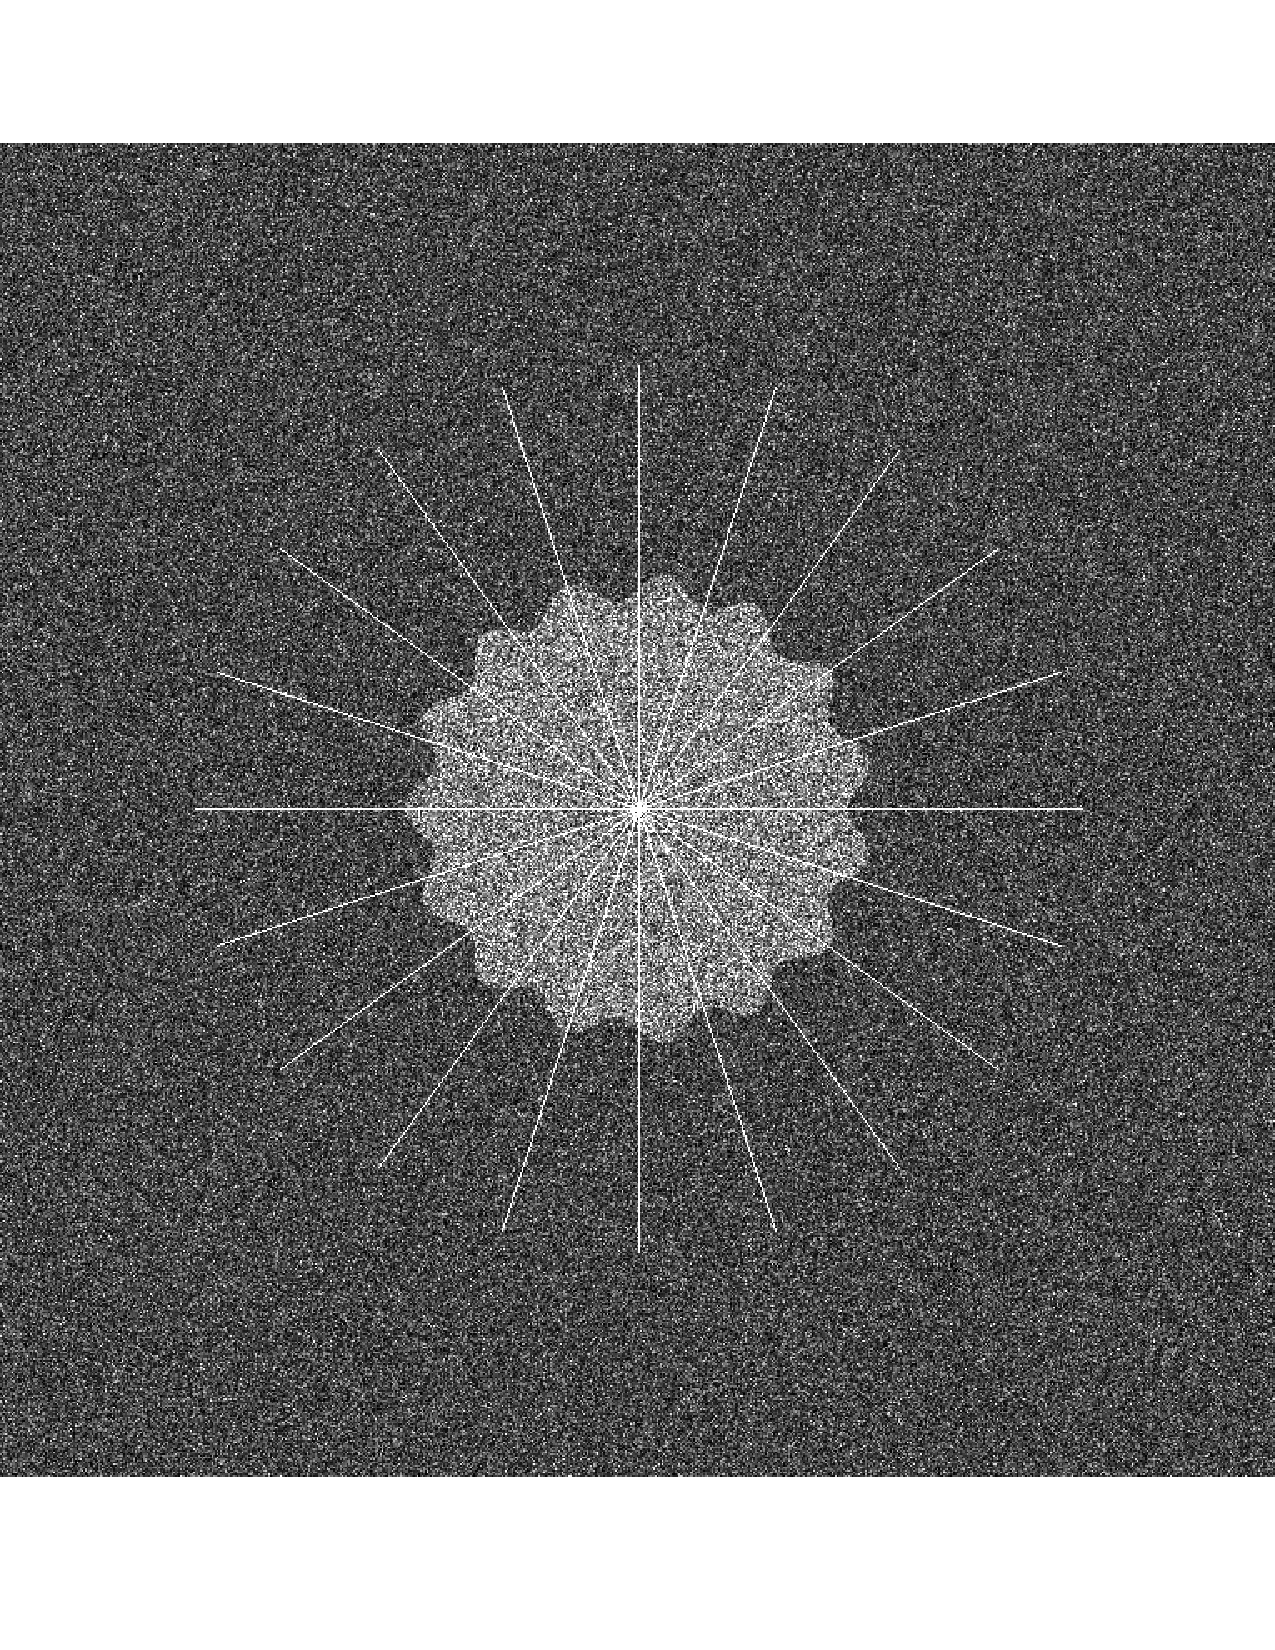
\includegraphics[width=\linewidth]{flor_15_133_8_hv.pdf}}
	\caption{Imagem flor simulada canal $I_{hv}$ com $\beta = 15$, $\delta = 133$ e $\nu = 8$ .}
\endminipage\hfill
\centering
\minipage{0.3\textwidth}
\fbox{ 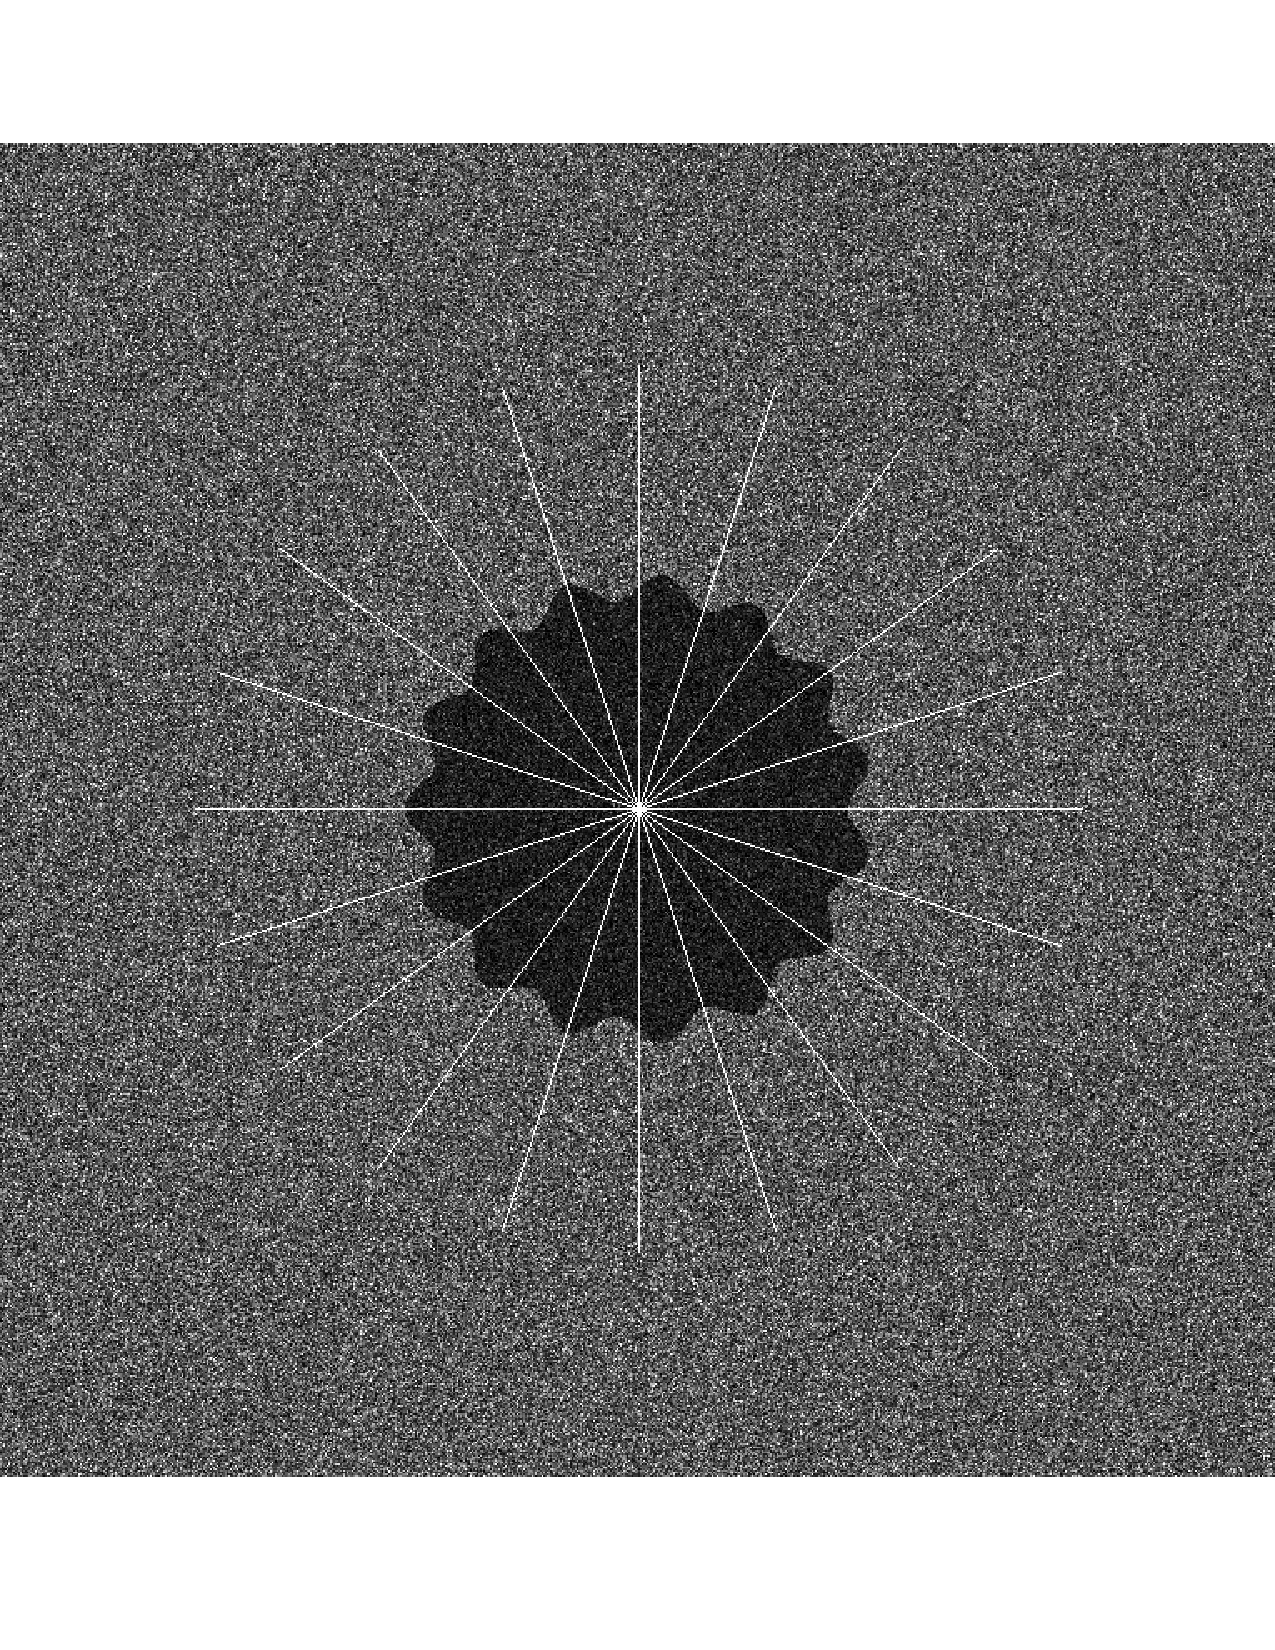
\includegraphics[width=\linewidth]{flor_15_133_8_vv.pdf}}
	\caption{Imagem flor simulada canal $I_{vv}$ com $\beta = 15$, $\delta = 133$ e $\nu = 8$ .}
\endminipage\hfill
\end{figure}
 
\end{frame}

\begin{frame}{Resultados numéricos}
\begin{figure}[hbt]
	\fbox{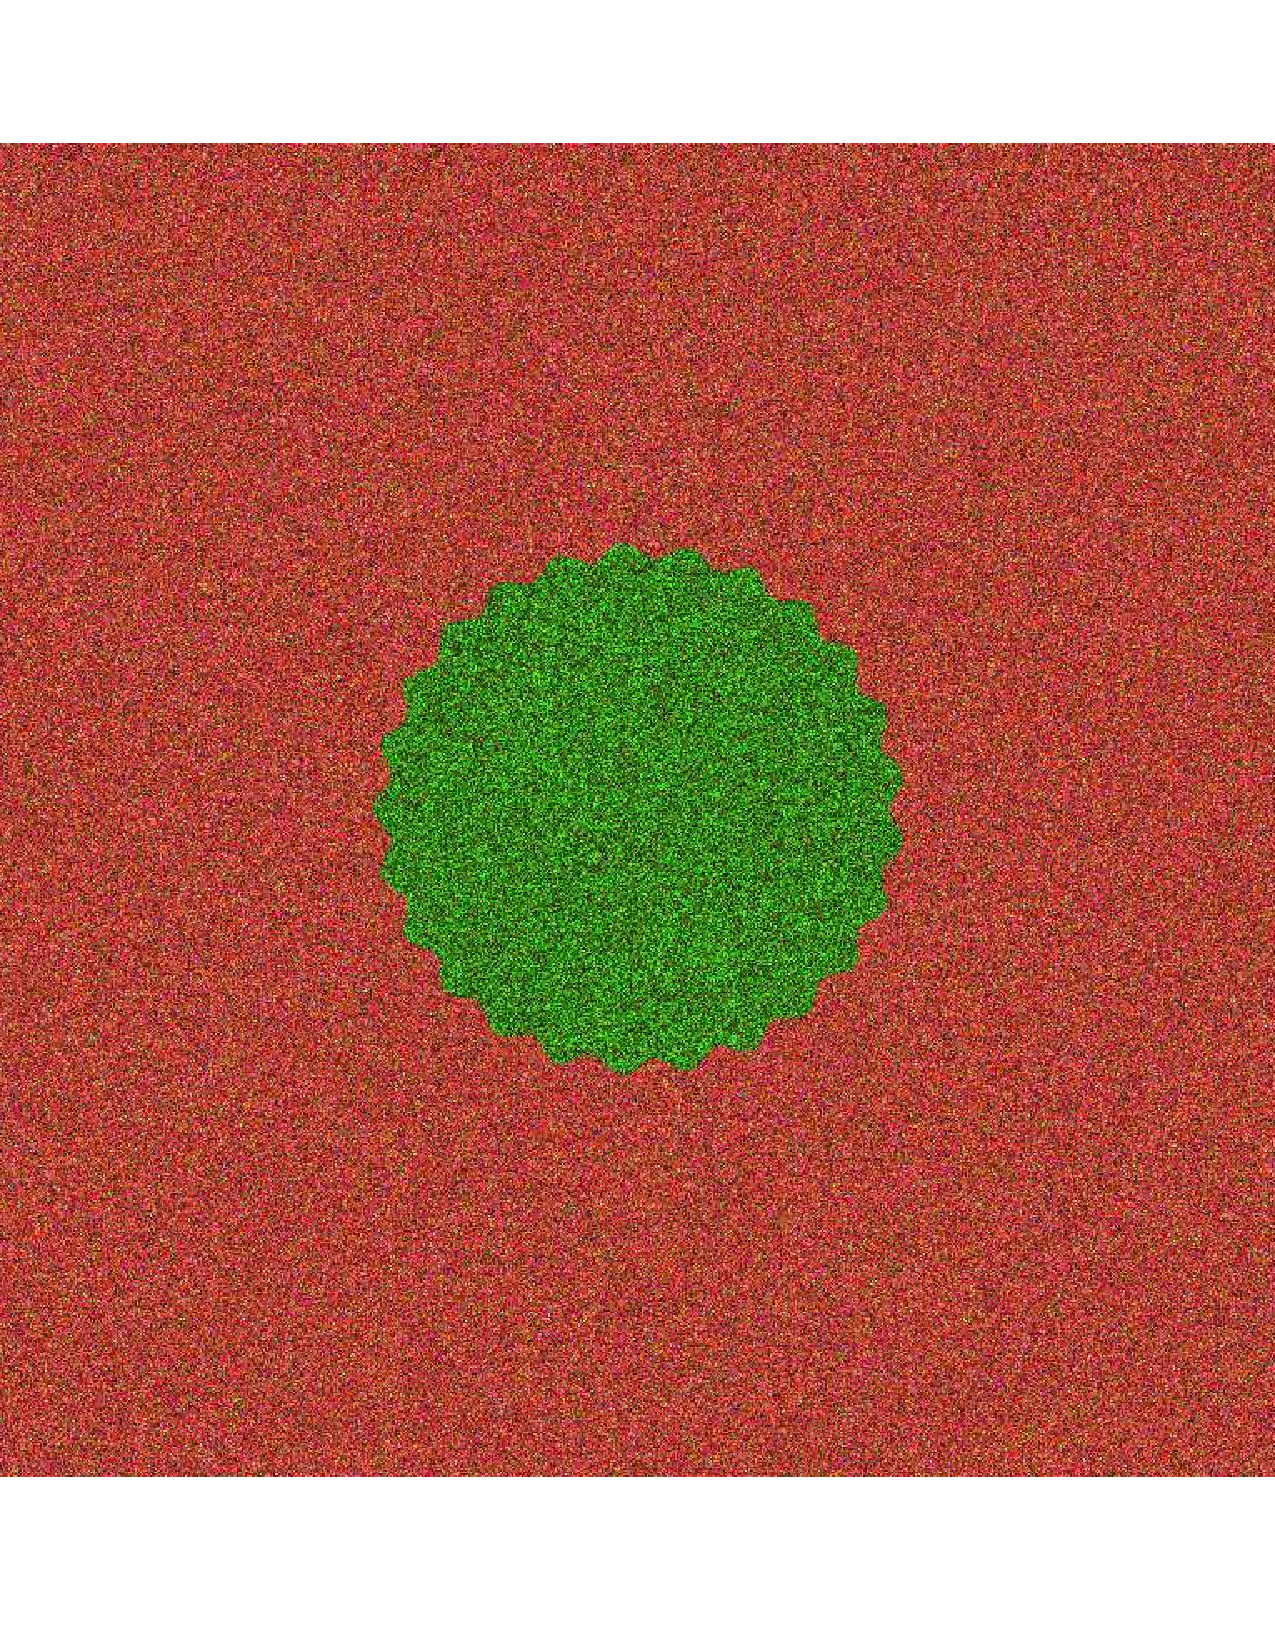
\includegraphics[scale=0.25]{flor_25_155_5_pauli.pdf}}
	\caption{Imagem flor simulada com $\beta = 25$, $\delta = 155$ e $\nu = 5$ .}
\label{cap_acf_fig15}
\end{figure}
\end{frame}

\begin{frame}{Resultados numéricos}
\begin{figure}[hbt]
\minipage{0.45\textwidth}
	\fbox{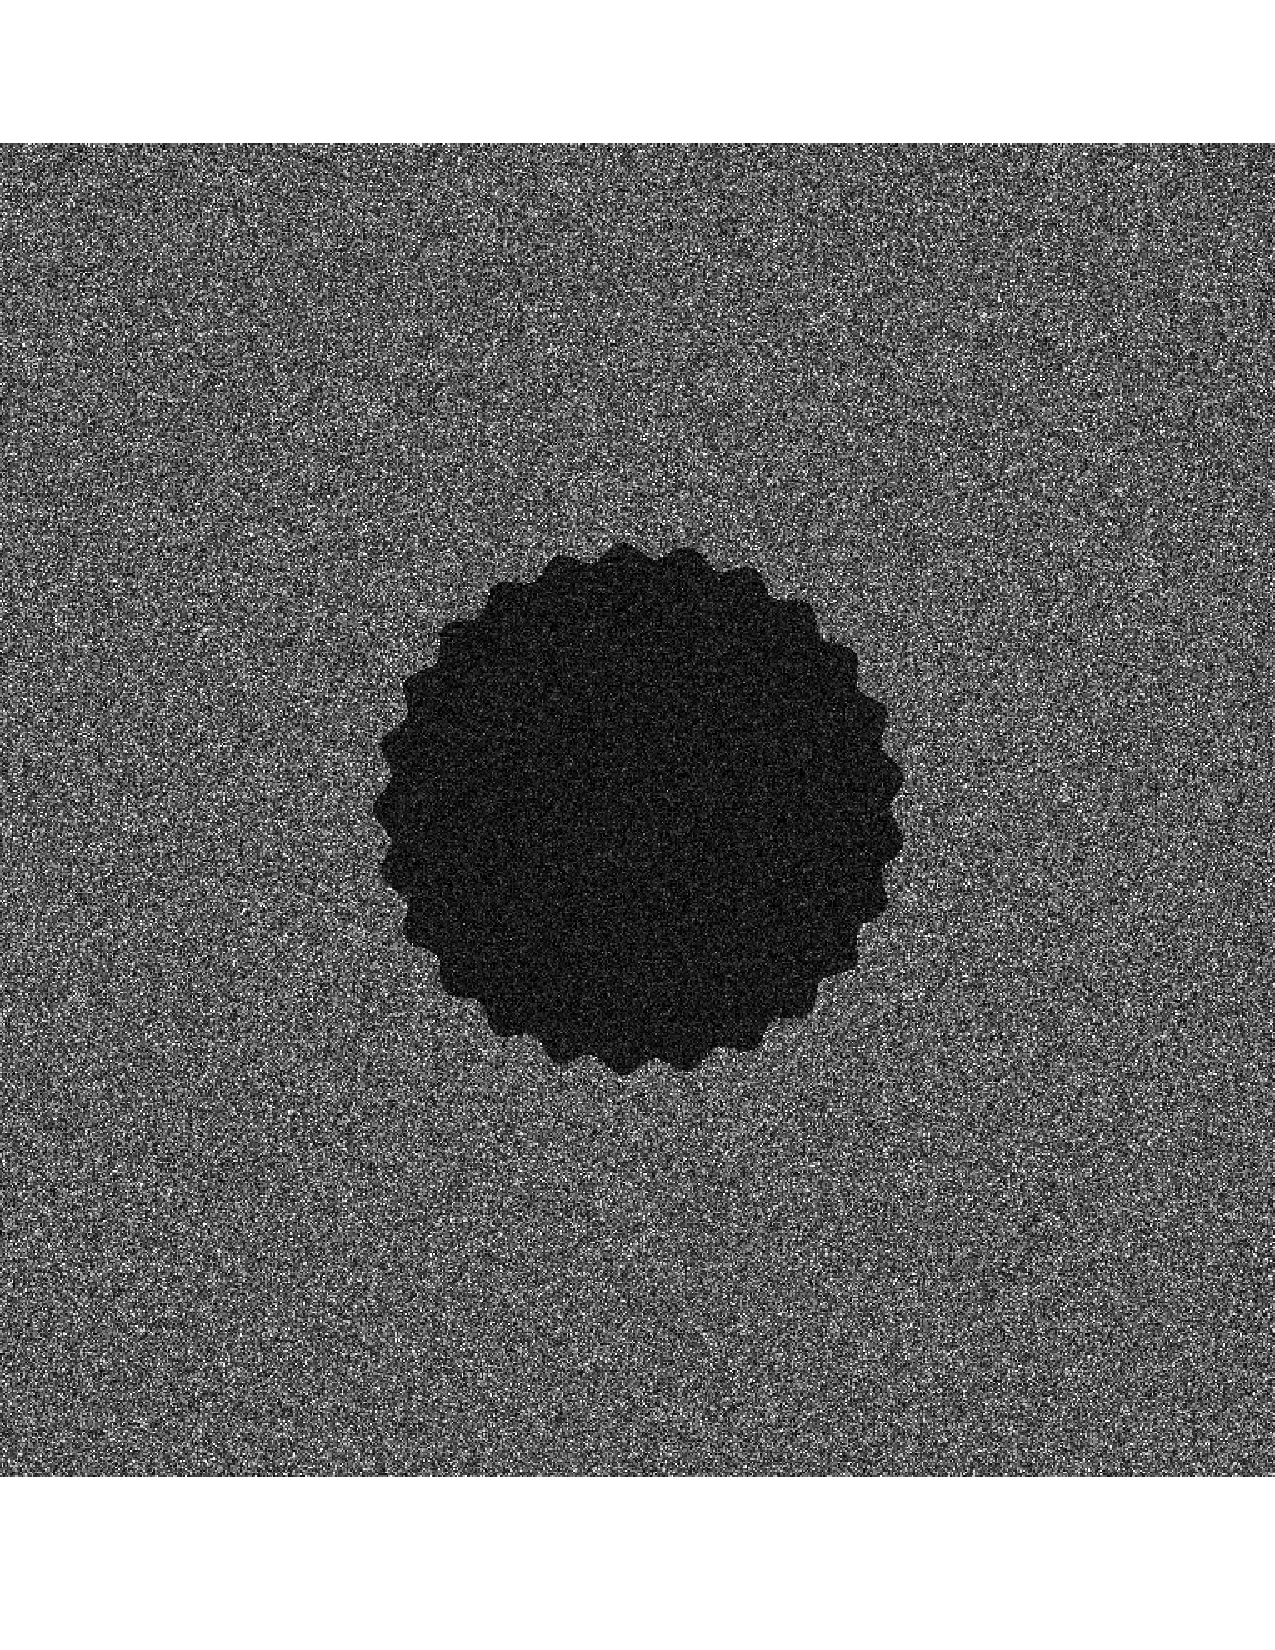
\includegraphics[width=\linewidth]{flor_25_155_5_hh.pdf}}
	\caption{Imagem flor simulada canal $hh$ com $\beta = 25$, $\delta = 155$ e $\nu = 5$ .}
\label{cap_acf_fig15}
\endminipage\hfill
\minipage{0.45\textwidth}
	\fbox{
\includegraphics[width=\linewidth]{flor_evid_25_155_5_hh.pdf}}
	\caption{Evidências de bordas canal $hh$ com $\beta = 25$, $\delta = 155$ e $\nu = 5$ .}
\label{cap_acf_fig16}
\endminipage\hfill
\end{figure}
\end{frame}
\begin{frame}{Resultados numéricos}
\begin{figure}[hbt]
\minipage{0.45\textwidth}
	\fbox{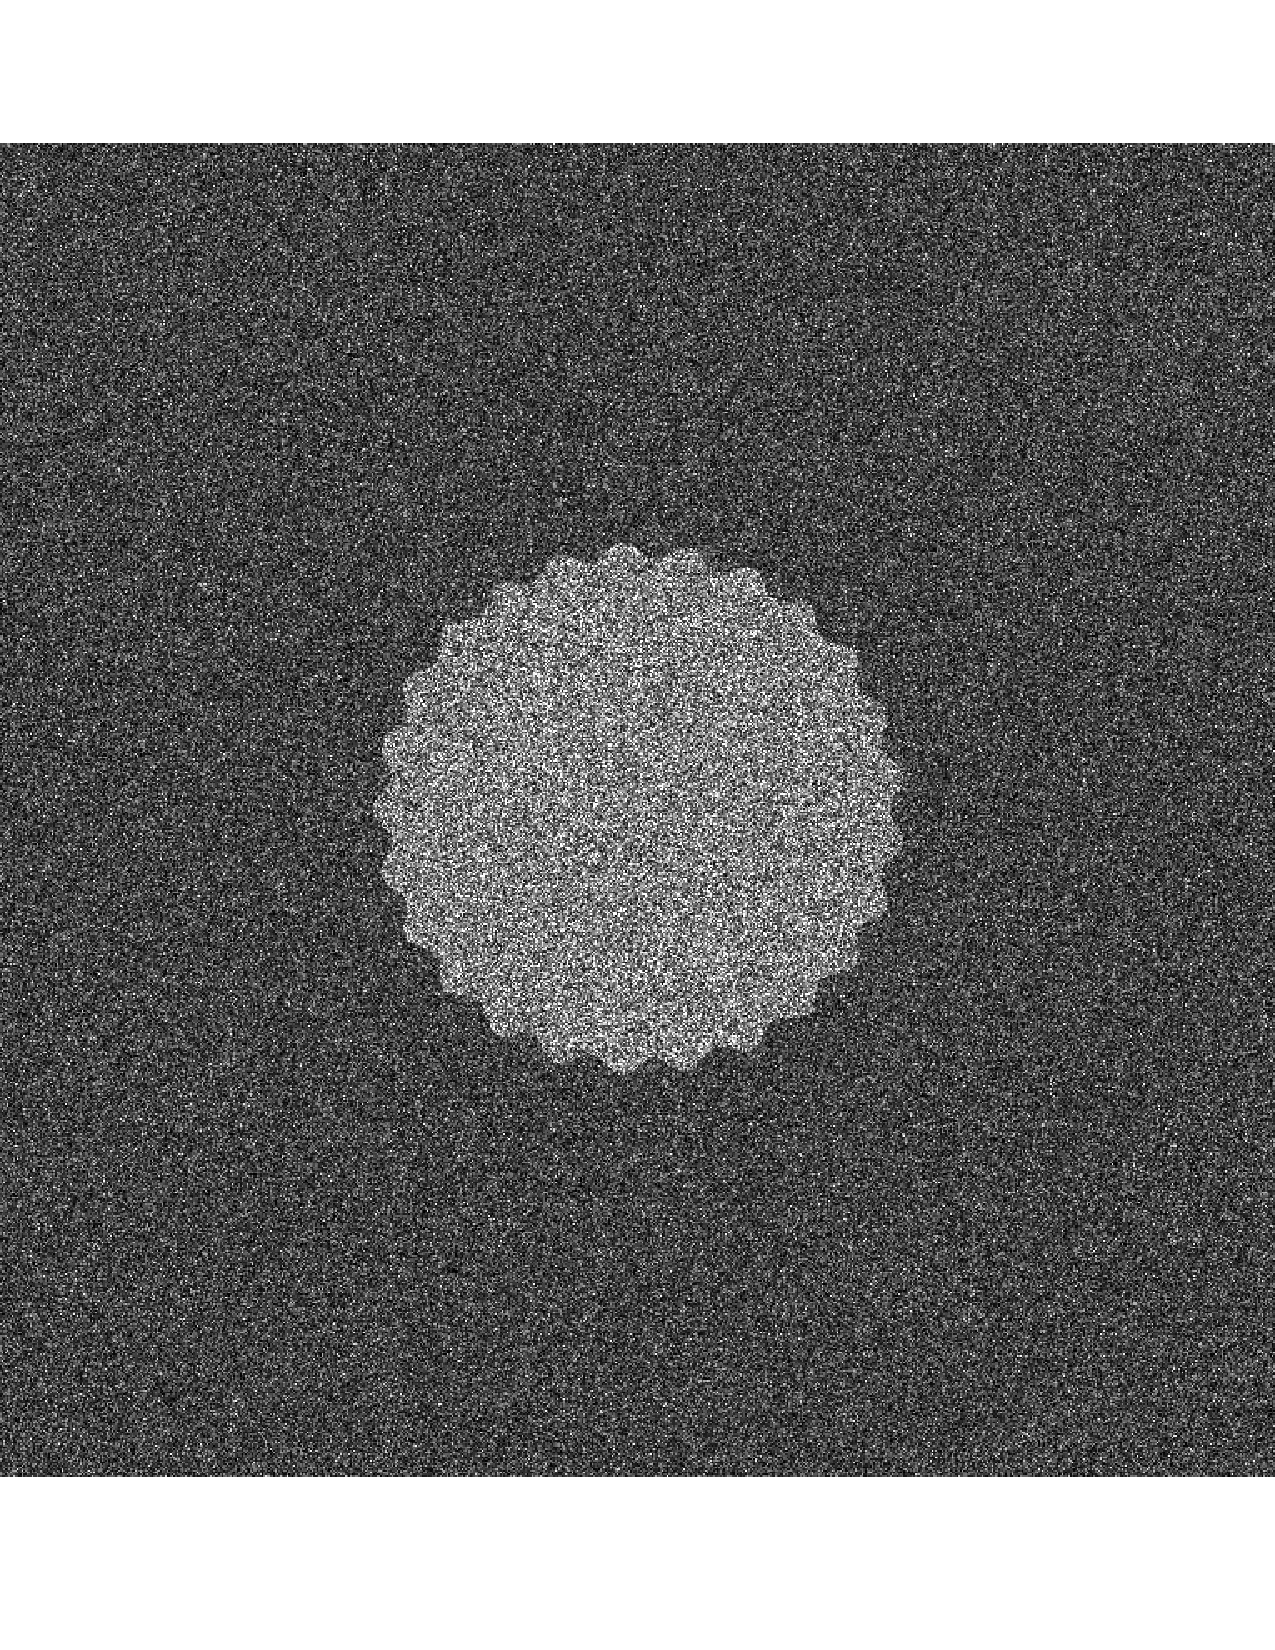
\includegraphics[width=\linewidth]{flor_25_155_5_hv.pdf}}
	\caption{Imagem flor simulada canal $hv$ com $\beta = 25$, $\delta = 155$ e $\nu = 5$ .}
\label{cap_acf_fig15}
\endminipage\hfill
\minipage{0.45\textwidth}
	\fbox{
\includegraphics[width=\linewidth]{flor_evid_25_155_5_hv.pdf}}
	\caption{Evidências de bordas canal $hv$ com $\beta = 25$, $\delta = 155$ e $\nu = 5$ .}
\label{cap_acf_fig16}
\endminipage\hfill
\end{figure}
\end{frame}
\begin{frame}{Resultados numéricos}
\begin{figure}[hbt]
\minipage{0.45\textwidth}
	\fbox{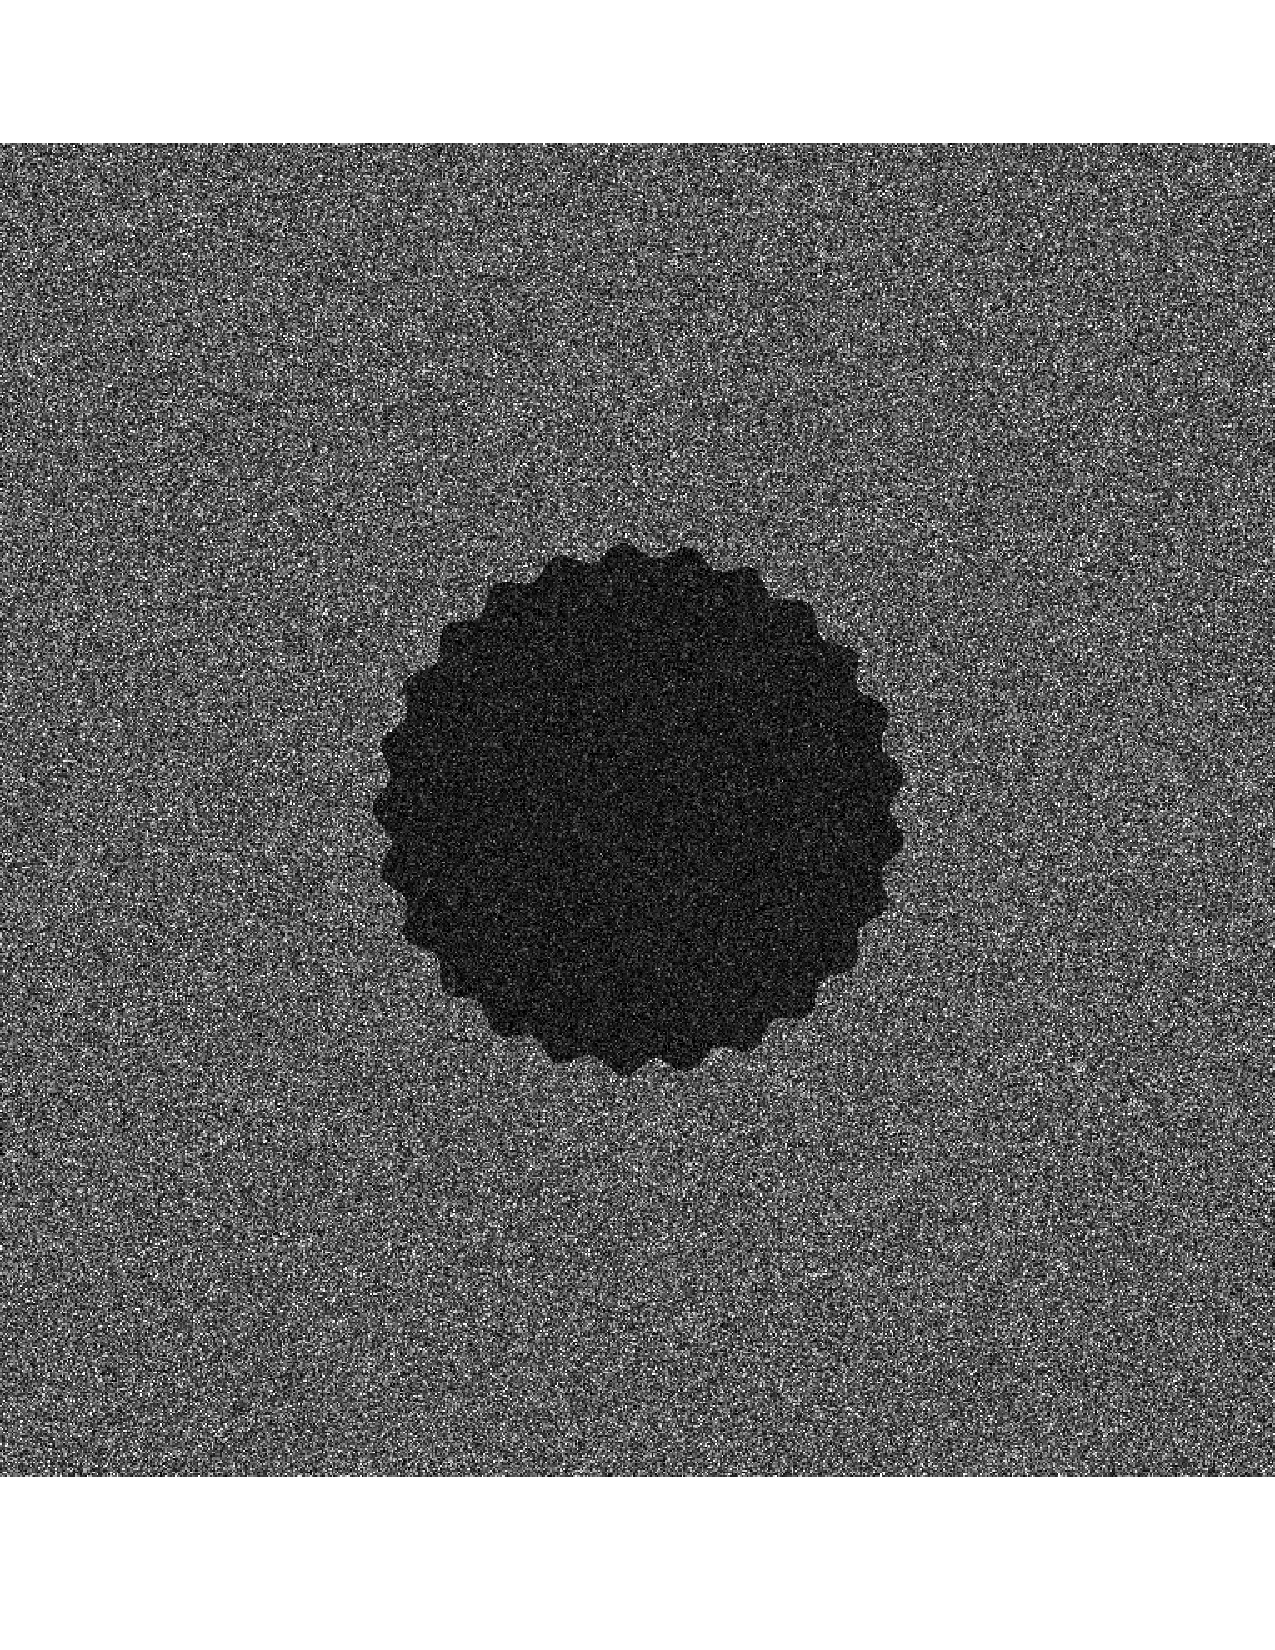
\includegraphics[width=\linewidth]{flor_25_155_5_vv.pdf}}
	\caption{Imagem flor simulada canal $vv$ com $\beta = 25$, $\delta = 155$ e $\nu = 5$ .}
\label{cap_acf_fig15}
\endminipage\hfill
\minipage{0.45\textwidth}
	\fbox{
\includegraphics[width=\linewidth]{flor_evid_25_155_5_vv.pdf}}
	\caption{Evidencias de bordas canal $vv$ com $\beta = 25$, $\delta = 155$ e $\nu = 5$ .}
\label{cap_acf_fig16}
\endminipage\hfill
\end{figure}

\end{frame}

%\begin{frame}{References}
%  Some references to showcase [allowframebreaks]\cite{knuth92,ConcreteMath,Simpson,Er01,greenwade93}
%\end{frame}

\section{Conclusão e trabalhos futuros}

\begin{frame}{Conclusão e trabalhos futuros}
\begin{alertblock}{Conclusão e trabalhos futuros}
\begin{itemize}
\item O método proposto mostrou ser eficiente na detecção de bordas com fusão de evidências;
\item Aplicar o método nas imagens simuladas;
\item Melhorar o método de fusão de evidências de bordas;
\item SVM, Randon Forest, CNN, PCA e análises estatísticas;
\item Aplicar em imagens reais.
\end{itemize}
\end{alertblock}
\end{frame}

\begin{frame}[standout]
  Sugestões ou perguntas?\\
  Obrigado!!!!
\end{frame}
\end{document}
